%----------------------------------------------------------------------------------------
%	CHAPTER 3 Cuantización de Campo Escalar
%----------------------------------------------------------------------------------------

\chapterimage{chapter_head_2.pdf}
\chapter{Cuantización de Campo Escalar}

\newcommand{\ON}{N}
\newcommand{\OH}{H}

\label{capitulo_3}

Habiendo tratado los aspectos necesarios de la teoría clásica de campos, vamos a comenzar a analizar las teorías cuánticas de campos relativistas. Para ello, comenzaremos estudiando la cuantización de teorías libres, es decir, de aquellas para las cuales no aparecen términos de interacción (o sea, términos con tres o más campos) en el Lagrangiano. Una de los motivos por los cuales las teorías libres son relevantes es porque se asume que en los procesos de scattering los estados asintóticos pueden ser descriptos por una teoría libre. Más allá de esto, el estudio de las teorías libres nos permitirá entender algunos aspectos de las teorías cuánticas de campos relativistas.\\

En esta primera parte utilizaremos el método de cuantización canónica. Sobre el final del curso
la idea es presentar otro método de cuantización, el de integrales de camino.\\

Tengan en cuenta que vamos a trabajar en la representación de Heisenberg de la mecánica cuántica: los operadores son los que evolucionan en el tiempo, mientras que los estados están
fijos.

\section{Cuantización canónica del campo escalar real}

Campo escalar es el campo relativista mas simple que se puede introducir. Estos campos se caracterizan por ser invariantes por transformaciones del grupo de Lorentz. De ahora en adelante, utilizaremos las unidades naturales descritas en el primer capitulo.

\subsection{Ecuación de movimiento}

Para derivar la ecuación de movimiento asociada a campo escalar, utilizaremos el análisis que permite derivar la ecuación de Schrödinger en mecánica cuántica
\begin{equation*}
    \ii \hbar \pdv{\psi(t,\vb*{x})}{t} = \qty[-\frac{\hbar^2}{2m}\laplacian + V(\vb*{x}) ] \psi(t,\vb*{x}),
\end{equation*}
que es la versión a nivel de operador de la relación asociada a la energía no relativista
\begin{equation*}
    \hat{E} = \frac{\hat{p}^{2}}{2m} + \hat{V}(\vb*{x}),
\end{equation*}

aplicada a la función de onda $\psi(t,\vb*{x})$ con
\begin{equation}
    \hat{E} \to \ii \hbar \pdv{t}, \quad\quad \hat{p} \to \ii\hbar \grad \, ,
\end{equation}

representaciones de los operadores energía y momento respectivamente. Ahora en el caso relativista se parte de la relación energía-momento relativista que en forma de operador se expresa como

\begin{IEEEeqnarray}{rCl}
    \hat{p}^{\mu}\hat{p}_{\mu} & = & m^{2} \implies \hat{p}^{\mu}\hat{p}_{\mu}-m^{2} =0 \, ,    \label{eq_3.1}
\end{IEEEeqnarray}
donde $m$ denota la masa de la partícula libre en reposo. Este operador deberá actuar sobre el campo $\phi (x)$ considerando a $\hat{p}_\mu \to \ii \partial_\mu$ como la representación del operador momento.\\

Teniendo en cuenta que 

\begin{equation*}
    \hat{p}_\mu \hat{p}^\mu = - \partial_\mu \partial^\mu = -\square \, , 
\end{equation*}

se obtiene la relación

\begin{IEEEeqnarray}{rCl} 
    \left( -\partial ^{\mu }\partial _{\mu }-m^{2}\right) \phi \left( x\right) &=&0  \label{eq_3.3} \\
    \left(\square ^{2}+m^{2}\right) \phi \left( x\right) &=&0  \notag
\end{IEEEeqnarray}

que es conocida como la ecuación de Klein-Gordon (EKG). Esta EKG describe el campo en ausencia de fuente, es decir, sin interacción. El hecho que la EKG sea la versión a nivel de operador del la relación energía momento $ p^{\mu}p_{\mu}= m^{2}$, indica que todo campo relativista deberá satisfacer esta expresión.\\

A simple vista, la EKG parece simple, pero hay un problema, los valores propios de energía son

\begin{equation} 
    p^{\mu}p_{\mu} = m^{2} \quad \implies \quad E^{2}=\vb*{p}^{2}+m^{2}  \quad \implies \quad E = \pm  \sqrt{\vb*{p}^2+m^2}.
    \label{eq_3.4}
\end{equation}

Aquí se tiene que la energía puede ser negativa y su magnitud puede ser arbitrariamente grande ya que $\abs{\vb*{p}}$ no está acotado. Por tanto, el sistema no tendrá estado fundamental y colapsará en valores de energía negativos cada vez mayores y será totalmente inestable. Por tanto, no es posible una interpretación de la función de onda de la EKG. Este problema tendrá una interpretación solo al cuantizar el campo.

\subsection{Cuantización canónica}

La EKG es la correspondiente ecuación de Euler-Lagrange derivada de la densidad Lagrangiana asociada a campo escalar $\phi (x)$, 

\begin{equation}
	\boxed{
    \mathcal{L}=\frac{1}{2}\left( \partial ^{\mu }\phi \right) \left( \partial_{\mu }\phi \right) -\frac{1}{2}m^{2}\phi ^{2} } \, ,
    \label{eq_3.5}
\end{equation}

la cual verifica que

\begin{equation}
    \pdv{\lagdn}{\phi}-\partial_{\mu}\pdv{\lagdn}{\qty(\partial_\mu \phi)}=0 \quad \implies \quad \left(\square^{2}+m^{2}\right) \phi (x) = 0~.
\end{equation}

Al extender la teoría al formalismo Hamiltoniano, se introduce el momento canónico conjugado asociado al campo $\phi$ como siendo

\begin{equation}
    \Pi(x) = \pdv{\lagdn}{\dot{\phi}} = \pdv{\lagdn}{\qty(\partial _{0}\phi)}.
    \label{eq_3.6}
\end{equation}

Empleando la densidad lagrangiana (\ref{eq_3.5}), se tiene que

\begin{IEEEeqnarray}{rCl}
    \Pi (x) &=& \pdv{\qty(\partial_0 \phi)}\qty\bigg[\frac{1}{2} \partial ^{\mu }\phi \partial_{\mu }\phi] \nonumber\\*
    & = & \partial^\mu \phi \pdv{\qty(\partial_\mu \phi)}{\qty(\partial_0 \phi)} = \partial^\mu \phi \delta^0_\mu \nonumber\\*
    & = & \partial^0 \phi = \dot{\phi} (x) \, .
    \label{eq_3.8}
\end{IEEEeqnarray}

El Hamiltoniano canónico asociado a campo escalar real clásico es 

\begin{IEEEeqnarray}{rCl}
    H & = & \int \dd[3]{x} \hamdn = \int \dd[3]{x} \qty\big[\dot{\phi}(x)\Pi (x)-\lagdn],
\end{IEEEeqnarray}
donde
\begin{IEEEeqnarray}{rCl}
    \hamdn &=& \dot{\phi}\Pi-\qty[\frac{1}{2}\partial^\mu\phi \partial_\mu\phi - \frac{1}{2} m^2 \phi^2] \nonumber\\*
    & = & \Pi \Pi-\frac{1}{2}\dot{\phi}\dot{\phi} +\frac{1}{2}\partial^k\phi \partial^k\phi - \frac{1}{2} m^2 \phi^2] \nonumber\\*
    & = & \frac{1}{2}\qty\bigg[\Pi^2+\qty(\grad \phi)^2 + m^2 \phi^2].
    \label{eq_3.10}
\end{IEEEeqnarray}

En mecánica clásica la evolución temporal de una variable dinámica se escribe en términos de su paréntesis de Poisson (PP) entre la variable y el Hamiltoniano canónico. Al generalizar la definición de corchete de Poisson para contemplar el caso en el cual tenemos grados de libertad continuos, introducimos lo que se conoce como derivada funcional, generalización trabajada en el capitulo \ref{capitulo_22}. Así los PP fundamentales a tiempos iguales entre las variables $\phi(x) \equiv \phi(t,\vb*{x})$ y $\Pi(x) \equiv \Pi(t,\vb*{x})$ son 

\begin{IEEEeqnarray}{rCl}
    \{ \phi(x),\Pi(y)\} &=& \delta^3(\vb*{x}-\vb*{y}) , \\
    \{ \phi(x),\phi(y)\} &=& 0 , \\
    \{ \Pi(x),\Pi(y)\} & = & 0.
\end{IEEEeqnarray}

Este es el punto de partida de la cuantización canónica que se introduce en Mecánica cuántica. El principio de correspondencia establece que $\{~,~\} \to \frac{1}{\ii \hbar}\comm{~}{~}$. En unidades naturales $\hbar=1$. Vamos a introducir los campos cuánticos hermíticos $\hat{\phi} \equiv \phi $ y $\hat{\Pi} \equiv \Pi$ que cumplen las siguientes relaciones de conmutación a tiempos iguales 

\newcommand{\Ophi}{\phi} % Operador \phi
\newcommand{\OPi}{\Pi} % Operador \Pi

\begin{IEEEeqnarray}{rCl}
    \comm{\Ophi(x)}{\OPi(y)} & = & \comm{\Ophi(t,\vb*{x})}{\OPi(t,\vb*{y})} = \ii \delta^3(\vb*{x}-\vb*{y}) \label{eq_3.14} ,\\
    \comm{\Ophi(x)}{\Ophi(y)} & = & \comm{\Ophi(t,\vb*{x})}{\Ophi(t,\vb*{y})} = 0 \label{eq_3.15} ,\\
    \comm{\OPi(x)}{\OPi(y)} & = & \comm{\OPi(t,\vb*{x})}{\OPi(t,\vb*{y})} = 0 \, . \label{eq_3.16}  
\end{IEEEeqnarray}

Lo anterior define las relaciones de conmutación canónica, lo que implica que $\phi $ y $\Pi $ ya no pueden ser considerados como campos clásicos. Ahora deben ser tratados como operadores cuánticos. El
procedimiento de cuantización es una consecuencia directa de esta relación de conmutación, como veremos gradualmente.\\

Aunque estamos tratando de construir una teoría covariante relativista, la relación de conmutación de (\ref{eq_3.14}) no parece ser una ecuación covariante, pues de cierto modo da un trato preferencial al componente de tiempo y por lo tanto no puede ser válido en un marco de referencia general. Sin embargo la ecuación (\ref{eq_3.14}) puede ser v\'{a}lida en cualquier marco de referencia. Observe que los PP conllevan a que el conmutador sea distinto de cero solo si consideramos el campo $\Ophi $ y el momento canónico $\OPi$ en el mismo punto espacio-temporal. Si dos puntos del espacio-tiempo coinciden en un marco, coincidirán en cualquier otro marco. Así, al menos para esta parte, no hay diferencia si pasamos a cualquier otro marco de referencia.\\

Una forma de ver esto es observando la transformación del conmutador aplicando una transformación de Lorentz al lado izquierdo del conmutador (\ref{eq_3.14}). Dado que $\phi$ es un escalar y $\Pi =\dot{\phi}=\partial_{0}\phi$, la propiedad de transformación de Lorentz no trivial del lado izquierdo proviene solo del término $\partial_{0}$. En otras palabras, el lado izquierdo se transforma como el componente de tiempo de un cuadrivector. En cuanto al lado derecho, observe que el término $\dd[4]{x} \delta^{3}(\vb*{x}-\vb*{y})$ resulta ser $dt$ al ser integrado sobre una región espacial en la cual $\vb*{x}=\vb*{y}$. Por definición $dt$ se transforma como el componente de tiempo de un cudrivector, y siendo $\dd[4]{x}$ una cantidad escalar, se debe cumplir que $\delta^{3}(\vb*{x}-\vb*{y})$ se transforme como el componente de tiempo de un cuadrivector. Por tanto la ecuación (\ref{eq_3.14}) es covariante.


\subsection{Análisis de Fourier para campo escalar}  \label{Cap_3 Subsección: Análisis de Fourier para campo escalar}

Al cuantizar canónicamente, el Hamiltoniano cuántico quedara con la misma forma prescrita clásicamente, solamente ahora se reemplaza los campos clásicos por sus versiones cuánticas

\begin{equation}
	\boxed{
    H = \int \dd[3]{x} \frac{1}{2}\qty[\OPi^2+\qty\big(\grad \Ophi)^2+m^2\phi^2]} \, .
    \label{eq_3.17}
\end{equation}

Sin embargo, pueden aparecer problemas asociados al orden de los operadores y tendremos que dar una prescripción para construir el Hamiltoniano cuántico. Vamos a ver que hay mucho en común entre el oscilador armónico y esta teoría de campos.\\ 

\newcommand{\CA}{\mathcal{A}} % Operador \Pi
\newcommand{\OCA}{\mathcal{A}}

Dado un campo clásico que es una función de las coordenadas del espacio-tiempo, puede determinarse que la transformada de Fourier de $\CA(p)$ es dada por el campo escalar $\phi(x)$ en la forma, 

\begin{equation}
    \phi \left( x\right) =\frac{1}{(2\pi)^{3/2}}\int \dd[4]{p} \delta (p^{2}-m^{2}) \CA \left(p\right) \ee^{-\ii px}, 
    \label{eq_3.18}
\end{equation}

donde el factor fuera del signo integral es solo un factor de normalización. Dentro de la integral, además de las habituales componentes de la T.F de $\CA(p)$, hemos puesto un factor $\delta^4(p^{2}-m^{2})$, el cual garantiza que $\phi$ cumpla la EKG. (La solución en TF satisface la ecuación homogénea de KG).\\

Para corroborar lo anterior considere la acción de operador $(\square^{2}+m^{2})$ sobre el campo $\phi(x)$,

\begin{IEEEeqnarray}{rCl}
    \qty(\square^{2}+m^{2})\phi(x) & = & \frac{1}{(2\pi)^{3/2}} \qty(\square^{2}+m^{2}) \int \dd[4]{p} \delta \left( p^{2}-m^{2}\right) \CA(p) \ee^{-\ii px} \nonumber\\*
    & = & \frac{1}{(2\pi)^{3/2}} \int \dd[4]{p} \delta \left( p^{2}-m^{2}\right) \CA(p)  \qty(\partial_\mu \partial^\mu) \ee^{-\ii px} \nonumber\\*
    && +\> \frac{m^{2}}{(2\pi)^{3/2}} \int \dd[4]{p} \delta \left( p^{2}-m^{2}\right) \CA(p) \ee^{-\ii px},
     \label{eq_3.19}
\end{IEEEeqnarray}
donde 
\begin{equation*}
    \begin{split}
        \partial_\mu \partial^\mu \ee^{-\ii px} &= - \ii \partial_\mu \ee^{-\ii px} \cancelto{p^\mu}{\partial^\mu(px)}\\
        & = -\ii p^\mu \partial_\mu \ee^{-\ii px} = -p^\mu p_\mu \\
        & = - p^2.
    \end{split} 
\end{equation*}
que al reemplazar en (\ref{eq_3.19}) implica:

\begin{IEEEeqnarray}{rCl}
    \qty(\square^{2}+m^{2})\phi(x) & = & -\frac{1}{(2\pi)^{3/2}} \int \dd[4]{p} \delta \left( p^{2}-m^{2}\right) \CA(p) \ee^{-\ii px} p^2  \nonumber\\*
    && +\> \frac{m^{2}}{(2\pi)^{3/2}} \int \dd[4]{p} \delta \left( p^{2}-m^{2}\right) \CA(p) \ee^{-\ii px} \nonumber\\*
    & = & \frac{1}{(2\pi)^{3/2}} \int \dd[4]{p} \qty(-p^{2} + m^{2}) \delta \left( p^{2}-m^{2}\right) \CA(p) \ee^{-\ii px} \quad \text{(Prop. Delta de Dirac)} \nonumber\\*
    & = & \frac{1}{(2\pi)^{3/2}}  \qty(-m^{2} + m^{2}) \eval{\CA(p) \ee^{-\ii px}}_{p^2 = m^2} = 0.
    \label{eq_3.20}
\end{IEEEeqnarray}

El resultado anterior se satisface gracias al factor introducido por el Delta de Dirac, garantizando que $\phi \left(x\right)$ sea solución a la EKG y a su ves al problema de partícula libre.\\

Introduciendo el operador hermítico\footnote{Clásicamente un operador hermítico significa que valor del campo en cualquier punto es un número real.} $\Ophi \left(x\right) $, la condición de hermiticidad hace que  $\Ophi(x)=\Ophi^{\dagger}(x)$. Por lo tanto en términos de la transformada de Fourier los operadores de campo bisónicos son

\begin{equation}
    \Ophi \left(x\right) =\frac{1}{(2\pi)^{3/2}}\int \dd[4]{p} \delta (p^{2}-m^{2}) \OCA \left(p\right) \ee^{-\ii px}, 
    \label{eq_3.21}
\end{equation}
y 
\begin{equation}
    \Ophi^{\dagger}\left(x\right) =\frac{1}{(2\pi)^{3/2}}\qty\bigg[\int \dd[4]{p} \delta (p^{2}-m^{2}) \OCA \left(p\right) \ee^{-\ii px}]^{\dagger}. 
    \label{eq_3.22}
\end{equation}

Estudiando este último término tenemos que 
\begin{equation*}
    \Ophi^{\dagger}\left(x\right) =\frac{1}{(2\pi)^{3/2}} \int \dd[4]{p} \delta (p^{2}-m^{2}) \OCA^{\dagger} \left(p\right) \ee^{+\ii px} \, ,
\end{equation*}

Al hacer un cambio de variable en la integral tal que $p^{\prime}=-p$, tenemos que $p \to \pm\infty \implies p^{\prime} \to \mp \infty$, además
\begin{IEEEeqnarray*}{rCl}
    \dd[4]{p} = \dd p^{0} \dd p^{1} \dd p^{2} \dd p^{3} & = & \qty(-\dd p^{\prime 0}) \qty(-\dd p^{\prime 1})\qty(-\dd p^{\prime 2}) \qty(-\dd p^{\prime 3}) \\ 
     & = & \dd p^{\prime 0} \dd p^{\prime 1} \dd p^{\prime 2} \dd p^{\prime 3}\\
     & = & \dd[4]{p^\prime}.
\end{IEEEeqnarray*}

Por lo tanto

\begin{IEEEeqnarray}{rCl}
    \Ophi^{\dag}(x) & = & \frac{1}{(2\pi)^{3/2}} \int \dd[4]{p^\prime} \delta \qty(p^{\prime 2}-m^2) \OCA^{\dagger} \left(-p^{\prime}\right) \ee^{-\ii p^{\prime}x} \quad (\text{redefinir } p^\prime=p) \notag\\
    & = &  \frac{1}{(2\pi)^{3/2}} \int \dd[4]{p} \delta \qty(p^{2}-m^2) \OCA^{\dagger} \left(-p\right) \ee^{-\ii px}.
    \label{eq_3.23}
\end{IEEEeqnarray}

Este resultado muestra que si $\Ophi(x)=\Ophi^{\dag}(x)$, entonces se cumple que

\begin{equation}
    \OCA^{\dagger} (-p) = \OCA(p) \quad \implies \quad \OCA^{\dagger} (p) = \OCA(-p). 
    \label{eq_3.24}
\end{equation}

Ahora, vamos a introducir la función Heaviside $\Theta \left( z\right)$, definida para cualquier variable real $z$ como:

\begin{equation}
    \Theta \left( z\right) =\left\{ \begin{array}{c} 
    1~\text{si}~z>0 \\ 
    1/2~\text{si}~z=0 \\ 
    0~\text{si}~z<0
    \end{array}
    \right.
    \label{eq_3.25}
\end{equation}

A partir de esta función, es posible establecer la identidad $\Theta(p^{0})+\Theta(-p^{0})=1$. Haciendo uso de este resultado en (\ref{eq_3.21}),


\begin{prof}
\begin{IEEEeqnarray*}{rCl}
    \Ophi \left(x\right) &=& \frac{1}{(2\pi)^{3/2}}\int \dd[4]{p} \delta (p^{2}-m^{2}) \OCA(p) \ee^{-\ii px}\qty[\Theta(p^{0})+\Theta(-p^{0})]\\
    & = & \frac{1}{(2\pi)^{3/2}}\int \dd[4]{p} \delta (p^{2}-m^{2}) \OCA(p) \Theta(p^{0}) \ee^{-\ii px} \\
    &&  +\> \frac{1}{(2\pi)^{3/2}}\int \dd[4]{p} \delta (p^{2}-m^{2}) \OCA(p) \Theta(-p^{0}) \ee^{-\ii px},
\end{IEEEeqnarray*}
nuevamente realizamos el cambio de variables $p=-p^{\prime}$ donde se verifica $\dd[4]{p}=\dd[4]{p^{\prime}}$, y cambiamos la variable de integración $p^{\prime}$ por $p$. En efecto se tiene que 
\begin{IEEEeqnarray*}{rCl}
    \Ophi \left(x\right) &=& \frac{1}{(2\pi)^{3/2}}\int \dd[4]{p} \delta (p^{2}-m^{2}) \OCA(p) \Theta(p^{0}) \ee^{-\ii px} \\
    &&  +\> \frac{1}{(2\pi)^{3/2}}\int \dd[4]{p} \delta (p^{2}-m^{2}) \OCA(-p) \Theta(p^{0}) \ee^{\ii px},
\end{IEEEeqnarray*}
finalmente al reemplazar (\ref{eq_3.24}) en el segundo término, demuestra:

\begin{equation}
	\boxed{
	\begin{IEEEeqnarraybox}{rCl}
		\Ophi \left(x\right) &=& \frac{1}{(2\pi)^{3/2}}\int \dd[4]{p} \delta (p^{2}-m^{2}) \Theta(p^{0}) \qty[\OCA(p)\ee^{-\ii px}+\OCA^{\dag}(p)\ee^{\ii px}]
		\label{eq_3.26}
	\end{IEEEeqnarraybox}
	} \, .
\end{equation}

\end{prof}

La característica de (\ref{eq_3.26}), es que al ser $p^0 = E$, los estados de energía asociados solo serán positivos.\\

De hecho, la transformada de Fourier se puede escribir en una forma algo simplificada si eliminamos $p^{0}$ de la Ec. (\ref{eq_3.26}). Para ello emplearemos la propiedad de la función delta de Dirac

\begin{cabox}
    La función delta de Dirac satisface la siguiente relación 
    \begin{equation}
    \delta\qty(f(z))= \sum_{k=1}^{n} \frac{\delta (z-c_{k})}{\abs{\eval*[\dv{f}{z}|_{z=c_k}}}, \quad \eval*[\dv{f}{z}|_{z=c_k}\neq 0, 
    \label{eq_3.27}
    \end{equation}
    donde $\{ c_k \}_{k=1}^{n}$ son todas las raices de la ecuación $g(z)=0$.
\end{cabox}

\begin{prof}
Considerando $f(z) = f(p^0)=p^2-m^2$, podemos hacer el siguiente análisis:

\begin{IEEEeqnarray*}{rCl}
    f(p^0) &=& \qty(p^0)^2 - \vb*{p}^2-m^2, \quad \text{(Considerando la energía relativista} \quad E_p ^2=\vb*{p}^2+m^2\text{)},\\
    &=& \qty(p^0)^2 - \qty(\vb*{p}^2 + m^2) = \qty(p^0)^2 - E_p ^2. 
\end{IEEEeqnarray*}

Luego, $f(p^0) = 0$, si
\begin{IEEEeqnarray*}{rCl}
    f(p^0) &=& \qty(p^0)^2 - E_p ^2 = \qty(p^0 - E_p)\qty(p^0 + E_p)=0\\
    && \implies \quad p^0=E_p \quad \text{y} \quad p^0=-E_p.
\end{IEEEeqnarray*}

Teniendo los puntos $c_k$, ahora se calcula la derivada de la función $f(p^{0})$, 

\begin{equation*}
    \dv{f}{p^0} = \dv{p^0} \qty[\qty(p^0)^2 - E_p ^2] = 2p^0.
\end{equation*}
 Así 
\begin{IEEEeqnarray}{rCl}
    \delta \qty(f\qty(p^0)) = \delta \qty(p^2 - m^2) &=& \delta \qty\bigg( \qty(p^0)^2 - E_p^2 ) \nonumber \\
    &=& \frac{1}{\abs{2E_p}}\qty\bigg[\delta \qty(p^0 - E_p) + \delta \qty(p^0 + E_p)],
    \label{eq_3.28}
\end{IEEEeqnarray}

donde $E_{p}$ representa el autovalor del operador de KG asociado a valores de energía positivos, es decir

\begin{equation}
    E_{p}=+ \sqrt{\vb*{p}^{2}+m^{2}}. 
    \label{eq_3.329}
\end{equation}
\end{prof}

Ahora, vamos a emplear el resultado (\ref{eq_3.28}) en la expresión asociada al operador del campo (\ref{eq_3.26}), de manera que

\begin{IEEEeqnarray*}{rCl}
    \Ophi \left(x\right) &=& \frac{1}{(2\pi)^{3/2}}\int \dd[4]{p} \frac{1}{\abs{2E_p}}\qty\bigg[\delta \qty(p^0 - E_p) 
    + \delta \qty(p^0 + E_p)] \Theta(p^{0}) \qty\bigg[\OCA(p)\ee^{-\ii px}+\OCA^{\dag}(p)\ee^{\ii px}]$ \IEEEeqnarraynumspace$ \\
    & = & \frac{1}{(2\pi)^{3/2}}\int \dd[4]{p} \frac{1}{\abs{2E_p}} \delta \qty(p^0 - E_p) \Theta(p^{0}) \qty\bigg[\OCA(p)\ee^{-\ii px}+\OCA^{\dag}(p)\ee^{\ii px}]  \\
    && +\>  \frac{1}{(2\pi)^{3/2}}\underbrace{\int \dd[4]{p} \frac{1}{\abs{2E_p}} \delta \qty(p^0 + E_p) \Theta(p^{0}) \qty\bigg[\OCA(p)\ee^{-\ii px}+\OCA^{\dag}(p)\ee^{\ii px}]}_0 \, ,
\end{IEEEeqnarray*}

observe el término $\delta \qty(p^0 + E_p) \Theta(p^{0})$ presente en la segunda integral permite evaluar $\eval{\Theta(p^{0})}_{p^0 =-E_p}$, y por la ecuación (\ref{eq_3.329}) $E_p$ es positivo ($\abs{E_p}=E_p$), lo que permite deducir $\eval{\Theta(p^{0})}_{p^0 = -E_p}=0$ y por tanto esta integral se anula. Así

\begin{IEEEeqnarray}{rCl}
    \Ophi \left(x\right) &=& \frac{1}{(2\pi)^{3/2}}\int \frac{\dd[4]{p}}{2E_p} \delta \qty(p^0 - E_p) \Theta(p^{0}) \qty\bigg[\OCA(p)\ee^{-\ii px}+\OCA^{\dag}(p)\ee^{\ii px}],
    \label{eq_3.30}
\end{IEEEeqnarray}

reescribiendo y resolviendo la integral aplicando la función delta de Dirac tenemos lo siguiente:

\begin{IEEEeqnarray}{rCl}
    \Ophi \left(x\right) &=& \int \frac{\dd[4]{p}}{\sqrt{2\qty(2\pi)^{3}E_p}} \frac{1}{\sqrt{2 E_p}}  \delta \qty(p^0 - E_p) \Theta(p^{0}) \qty\bigg[\OCA(p)\ee^{-\ii px}+\OCA^{\dag}(p)\ee^{\ii px}]\nonumber \\
    %%
    &=& \int \frac{\dd[3]{p}}{\sqrt{2\qty(2\pi)^{3}E_p}} \frac{1}{\sqrt{2 E_p}}  \int \dd{p^0} \delta \qty(p^0 - E_p) \Theta(p^{0}) \qty\bigg[\OCA(p)\ee^{-\ii px}+\OCA^{\dag}(p)\ee^{\ii px}],
    \label{eq_3.31}
\end{IEEEeqnarray}

donde el cálculo de la segunda integral se realiza como


\begin{prof}
	\begin{IEEEeqnarray*}{rCl}
      I &\equiv& \int \dd{p^0} \delta \qty(p^0 - E_p) \Theta(p^{0}) \qty\bigg[\OCA(p)\ee^{-\ii px}+\OCA^{\dag}(p)\ee^{\ii px}]\\
      &=&\int \dd{p^0} \delta \qty(p^0 - E_p) \Theta(p^{0}) \OCA(p)\ee^{-\ii px} \\
      && +\> \int \dd{p^0} \delta \qty(p^0 - E_p) \Theta(p^{0}) \OCA^{\dag}(p)\ee^{\ii px}, \quad \text{donde $p=(p^0,\vb*{p})$}\\
      &=&\int \dd{p^0} \delta \qty(p^0 - E_p) \Theta(p^{0}) \OCA(p^0,\vb*{p})\ee^{-\ii p^0 x^0}\ee^{+\ii \vb*{p} \cdot \vb*{x}} \\
      && +\> \int \dd{p^0} \delta \qty(p^0 - E_p) \Theta(p^{0}) \OCA^{\dag}(p^0,\vb*{p})\ee^{\ii p^0 x^0} \ee^{-\ii \vb*{p} \cdot \vb*{x}}, 
	\end{IEEEeqnarray*}

y al aplicar la función delta de Dirac la integral se reduce a

\begin{IEEEeqnarray}{rCl}
      I &=& \Theta(E_p) \OCA(E_p,\vb*{p})\ee^{-\ii E_p x^0}\ee^{+\ii \vb*{p} \cdot \vb*{x}} + \Theta(E_p) \OCA^{\dag}(E_p,\vb*{p})\ee^{\ii E_p x^0} \ee^{-\ii \vb*{p} \cdot \vb*{x}}. \label{eq_3.32}
\end{IEEEeqnarray}

\end{prof}

 Redefiniendo $p \equiv \qty(E_p,\vb*{p})$, y sabiendo que $\Theta(E_p)=1$, la ecuación (\ref{eq_3.31}) adquiere la forma

\begin{IEEEeqnarray}{rCl}
    \Ophi \left(x\right) &=& \int \frac{\dd[3]{p}}{\sqrt{2\qty(2\pi)^{3}E_p}} \frac{1}{\sqrt{2 E_p}} \qty\bigg[\OCA(p)\ee^{-\ii px} + \OCA^{\dag}(p)\ee^{\ii px}].
    \label{eq_3.33}
\end{IEEEeqnarray}

Al definir el nuevo operador

\begin{equation}
    \Oa_p \equiv \frac{\OCA(p)}{\sqrt{2E_p}},
\end{equation}

la expresión asociada al campo escalar (\ref{eq_3.33}) en términos de los operadores $a_p$ y $a^{\dagger}_p$ es

\begin{equation}
    \boxed{\Ophi \left(x\right) =  \int \frac{\dd[3]{p}}{\sqrt{2\qty(2\pi)^{3}E_p}} \qty\bigg[\Oa_p \ee^{-\ii px} + \Oa^{\dag}_p\ee^{\ii px}] } \, .
    \label{eq_3.35}
\end{equation}

%\begin{IEEEeqnarray}{rCl}
%    \Ophi \left(x\right) &=&  \int \frac{\dd[3]{p}}{\sqrt{2\qty(2\pi)^{3}E_p}} \qty\bigg[\Oa_p \ee^{-\ii px} + \Oa^{\dag}_p\ee^{\ii px}].
%    \label{eq_3.35}
%\end{IEEEeqnarray}

Con esta expresión (que nos resultará mas útil) asociada al campo $\Ophi$, el operador momento canónico conjugado se puede determinar empleando la definición (\ref{eq_3.8}), es decir

\begin{IEEEeqnarray}{rCl}
    \OPi(x) &=& \partial_0 \Ophi(x),
\end{IEEEeqnarray}
de este modo,

\begin{IEEEeqnarray}{rCl}
    \OPi(x) &=& \pdv{t} \int \frac{\dd[3]{p}}{\sqrt{2\qty(2\pi)^{3}E_p}} \qty\bigg[\Oa_p \qty\big(\ee^{-\ii px}) + \Oa^{\dag}_p\qty\big(\ee^{\ii px})] \notag \\
    & = & \int \frac{\dd[3]{p}}{\sqrt{2\qty(2\pi)^{3}E_p}} \qty\bigg[\Oa_p \pdv{t} \qty\big(\ee^{-\ii px}) + \Oa^{\dag}_p \pdv{t} \qty\big(\ee^{\ii px})]. \notag 
\end{IEEEeqnarray}
Pero al evaluar la derivada temporal,
\begin{equation*}
    \pdv{t} \qty\big(\ee^{\pm \ii px}) =\pm \ii \ee^{\pm \ii px} \cancelto{E_p}{\pdv{t}\qty(px)}= \pm \ii E_p \ee^{\pm \ii px},
\end{equation*}
así el operador momento canónico adquiere la forma 

\begin{equation}
    \boxed{\OPi(x)  =  -\ii \int \dd[3]{p} \sqrt{\frac{E_p}{2\qty(2\pi)^{3}}} \qty\bigg[\Oa_p \ee^{-\ii px} - \Oa^{\dag}_p \ee^{\ii px}].}
    \label{eq_3.37}
\end{equation}

A partir de las expresiones (\ref{eq_3.14}) a (\ref{eq_3.16}) es fácil demostrar las relaciones de conmutación entre $\Oa$ y $\Oa^\dag$ a tiempos iguales\footnote{($\Oa,\Oa^\dag$) son los operadores son evolucionar, a tiempo constante $t_0 = 0.$}, es decir


\begin{equation}
\boxed{
    \begin{IEEEeqnarraybox}{rCl}
        \comm{\Oa_p}{\Oa^\dagger_{p^\prime}} & = & \delta^3 \qty(\vb*{p}-\vb*{p^\prime}), \\
        \comm\big{\Oa_p}{\Oa_{p^\prime}} & = & 0. \\
        \comm{\Oa^\dagger_p}{\Oa^\dagger_{p^\prime}} & = & 0
    \end{IEEEeqnarraybox}
   } \, .
    \label{eq_3.38}
\end{equation}

Para demostrar estas relaciones es necesario tomar las transformadas inversas de Fourier de las expresiones (\ref{eq_3.35}) y (\ref{eq_3.37}) que nos permitirán escribir $\Oa(p)$ y $\Oa^{\dag}(p)$
en t\'{e}rminos de $\Ophi(x)$ y $\OPi(x)$. \\

\begin{prof}
	
Las reglas de conmutación (\ref{eq_3.38}) representan algo ya visto en el primer capitulo. Recuerde que los operadores de \emph{creación} y \emph{destrucción} de modos de energía $\hbar \omega$ de un oscilador armónico con un Hamiltoniano
\begin{equation}
    \OH = \frac{P^2}{2m}+\frac{1}{2} m \omega^2 X^2,
\end{equation}

puede solucionarse a partir de los operadores (ver ecs. (\ref{1.4a})) y (\ref{1.4b}))

\begin{equation}
    X =-\ii \sqrt{\frac{\hbar}{2m\omega}} \qty(\Oa-\Oa^\dag), \quad P = \sqrt{\frac{\hbar m \omega}{2}}\qty(\Oa+\Oa^\dag), 
\end{equation}
que satisfacen las reglas de conmutación 
\begin{equation}
    \comm{X}{P} = \ii \hbar \quad \implies \comm{\Oa}{\Oa^\dag} = 1,\quad \comm{\Oa}{\Oa}=\comm{\Oa^\dag}{\Oa^\dag}=0.
\end{equation}
De estas relaciones se demostró que

\begin{equation}
    \OH = \hbar \omega \qty\big(\Oa^\dag \Oa+ \frac{1}{2}),
\end{equation}
y que los conmutadores entre el operador Hamiltoniano $\OH$ y los operadores $(\Oa,\Oa^\dag)$ sean de la forma,

\begin{equation}
    \comm{\OH}{\Oa^\dag}=\hbar \omega \Oa^\dag, \quad \comm{\OH}{\Oa}=-\hbar \omega \Oa.
    \label{eq_3.43}
\end{equation}
Estos conmutadores permitieron darle una interpretación a $\qty(\Oa,\Oa^\dag)$. Además se definió el estado de mínima energía (\emph{el vacio}) $\ket{0}$ como aquél que es aniquilado por el operador $\Oa$, 

\begin{equation}
    \Oa \ket{0} = 0 \quad \implies \quad \Oa^\dag \Oa \ket{n} \equiv \ON \ket{n} = n \ket{n}, \quad \ket{n}=\frac{1}{\sqrt{n!}}\qty(\Oa^\dag)^n\ket{0},
\end{equation}

donde $\Oa^\dag \Oa=\ON$ es el operador número de modos. Se demostró que $\ket{0}$ tiene energía $E_0=\frac{1}{2}\hbar \omega$ y $\ket{n}$ tiene energía $E_{n}=\hbar \omega \qty(n+\frac{1}{2})$. Los auto estados $\qty{\ket{n}}$ del hamiltoniano asociado generan el espacio de Hilbert del sistema, llamado \emph{espacio de Fock}, sobre el cual ya hablaremos más adelante.\\

\end{prof}

Esta prescripción del oscilador armónico se extiende a teoría de campos, donde (\ref{eq_3.38}) son las relaciones de conmutación de un conjunto infinito de osciladores armónicos, uno por cada valor de $\vb*{p}$, excepto por un factor de normalización que es el volumen (infinito) del sistema, pues esta asociado con que ahora los grados de libertad son continuos,

\begin{equation}
    \lim_{\vb*{p}\to\vb*{p^\prime}} \delta^3\qty(\vb*{p}-\vb*{p^\prime}) = \lim_{\vb*{p} \to\vb*{p^\prime}} \int \frac{\dd[3]{x}}{\qty(2 \pi)^3} \ee^{\ii \vb*{x} \cdot \qty(\vb*{p}-\vb*{p^\prime})}= \frac{1}{\qty(2 \pi)^3} V(\to \infty).
\end{equation}

%Sin embargo, en la literatura se presentan resultados diferentes en (\ref{eq_3.38}), esto ocurre si se considera un prefactor diferente a $1/ \qty(2 \pi)^3/2$ en la ecuación (\ref{eq_3.18}), conllevando a que el lado derecho del conmutador entre $\Oa_p$ y $\Oa_p^{\dag}$ presente algunos factores adicionales.\\


%------------------------------------------
Ahora, vamos a partir de los conmutadores dados en (\ref{eq_3.38}) y la expansión de Fourier del campo $\Ophi(x)$ y $\OPi(x)$ para calcular el conmutador entre ellos, teniendo como punto de partida que se debe cumplir (\ref{eq_3.14}). De este modo

\begin{IEEEeqnarray*}{rCl}
    \comm{\Ophi \qty(t,\vb*{x})}{\OPi \qty(t,\vb*{y})} &=& \ii \int \frac{\dd[3]{p}}{\sqrt{2\qty(2\pi)^{3}E_p}}  \int \dd[3]{p^\prime} \sqrt{\frac{E_{p^\prime}}{2\qty(2\pi)^{3}}} 
    \comm{\qty\Big(\Oa_p \ee^{-\ii px} + \Oa^{\dag}_p \ee^{\ii px})}{\qty\Big(- \Oa_{p^\prime} \ee^{-\ii p^{\prime}y} + \Oa^{\dag}_{p^\prime} \ee^{\ii p^{\prime}y})}\\
    & = & \ii \int \int  \frac{\dd[3]{p} \dd[3]{p^\prime}}{2\qty(2 \pi)^3} \sqrt{\frac{E_{p^\prime}}{E_p}} \qty\Big(-\comm{\Oa^{\dag}_p}{\Oa_{p^\prime}} \ee^{\ii px} \ee^{-\ii p^{\prime}y} 
    + \comm{\Oa_p}{\Oa^{\dag}_{p^\prime}} \ee^{-\ii px} \ee^{\ii p^{\prime}y} ).
\end{IEEEeqnarray*}

%Esta ecuación implícitamente muestra que el conmutador $\comm{\Ophi \qty(t,\vb*{x})}{\OPi \qty(t,\vb*{y})}$ va a resultar en una función delta de Dirac debido a 

Aplicando las expresiones (\ref{eq_3.38}) y teniendo presente la propiedad  $\delta^3(-\vb*{z})=\delta^3(\vb*{z})$, tenemos:

\begin{prof}
	\begin{IEEEeqnarray*}{rCl}
		\comm{\Ophi \qty(t,\vb*{x})}{\OPi \qty(t,\vb*{y})} &=& \ii \int \int  \frac{\dd[3]{p} \dd[3]{p^\prime}}{2\qty(2 \pi)^3} \sqrt{\frac{E_{p^\prime}}{E_p}} \qty\Big(\delta^3 \qty(\vb*{p}-\vb*{p^\prime}) \ee^{\ii px} \ee^{-\ii p^{\prime}y} + \delta^3 \qty(\vb*{p}-\vb*{p^\prime}) \ee^{-\ii px} \ee^{\ii p^{\prime}y}) \\
		& = & \ii \int \int  \frac{\dd[3]{p} \dd[3]{p^\prime}}{2\qty(2 \pi)^3} \sqrt{\frac{E_{p^\prime}}{E_p}} \qty\Big(\ee^{\ii \qty(px - p^{\prime}y)} + \ee^{-\ii \qty(px - p^{\prime}y)} ) \delta^3 \qty(\vb*{p}-\vb*{p^\prime}) \\
		& = & \ii \int \int  \frac{\dd[3]{p} \dd[3]{p^\prime}}{2\qty(2 \pi)^3} \sqrt{\frac{E_{p^\prime}}{E_p}} \left( \ee^{\ii \qty(E_p - E_{p^\prime})t} \ee^{\ii\qty(-\vb*{p}\cdot\vb*{x}+\vb*{p^\prime}\cdot\vb*{y})}  \right. \\
		&& \quad +\> \left. \ee^{-\ii \qty(E_p - E_{p^\prime})t} \ee^{-\ii\qty(-\vb*{p}\cdot\vb*{x}+\vb*{p^\prime}\cdot\vb*{y})} \right) \delta^3 \qty(\vb*{p}-\vb*{p^\prime}) \\
		& = & \ii \int \frac{\dd[3]{p}}{2\qty(2 \pi)^3} \sqrt{\frac{E_{p}}{E_p}} \qty\Big( \ee^{-\ii \vb*{p}\cdot \qty(\vb*{x}-\vb*{y})} + \ee^{\ii \vb*{p}\cdot \qty(\vb*{x}-\vb*{y})}) \\
		& = & \frac{\ii}{2} \qty\Big( \int \frac{\dd[3]{p}}{\qty(2 \pi)^3} \ee^{-\ii \vb*{p}\cdot \qty(\vb*{x}-\vb*{y})} + \int \frac{\dd[3]{p}}{\qty(2 \pi)^3} \ee^{\ii \vb*{p}\cdot \qty(\vb*{x}-\vb*{y})}). 
	\end{IEEEeqnarray*}
\end{prof}

Y recordando que la función delta de Dirac se puede escribir como 

\begin{equation}
    \delta^3 \qty( \vb*{x}-\vb*{y})= \int \frac{\dd[3]{p}}{\qty(2\pi)^3} \ee^{\ii \vb*{p}\cdot\qty(\vb*{x}-\vb*{y})}, \quad  \delta^3 \qty( \vb*{x}-\vb*{y})=\delta^3 \qty( \vb*{y}-\vb*{x}),
    \label{eq_3.39}
\end{equation}
se obtiene

\begin{IEEEeqnarray}{rCl}
    \comm{\Ophi \qty(t,\vb*{x})}{\OPi \qty(t,\vb*{y})} &=& \frac{\ii}{2} \qty\Big(\delta^3 \qty( \vb*{x}-\vb*{y}) + \delta^3 \qty( \vb*{x}-\vb*{y})) = \ii \delta^3 \qty( \vb*{x}-\vb*{y}) \, .
    \label{eq_3.40}
\end{IEEEeqnarray}

Ya establecidos los operadores $\Ophi (x)$ y $\OPi (x)$ en términos de los operadores aniquilador y creador $\Oa$ y $\Oa^{\dagger}$, al igual que con el oscilador armónico conviene reescribir el Hamiltoniano planteado en (\ref{eq_3.17}), el cual permitirá ver cual es la energía de los estados multipartícula. Para derivar este Hamiltoniano debemos calcular cada uno de los términos planteados en la ecuación (\ref{eq_3.17}), así:
%---------------------------------------------------

\begin{IEEEeqnarray}{rCl}
    \int \dd[3]{x} \qty(\OPi(x))^2 & = & -\int \dd[3]{x} \dd[3]{p} \dd[3]{p^\prime} \sqrt{\frac{E_p}{2\qty(2\pi)^{3}}} \sqrt{\frac{E_{p^\prime}}{2\qty(2\pi)^{3}}} \qty\bigg(\Oa_p \ee^{-\ii px} - \Oa^{\dag}_p \ee^{\ii px}) \qty\bigg(\Oa_{p^\prime} \ee^{-\ii p^\prime x} - \Oa^{\dag}_{p^\prime} \ee^{\ii p^\prime x}), $\IEEEeqnarraynumspace$ 
    \label{eq_3.48}
\end{IEEEeqnarray}
donde la multiplicación entre los dos paréntesis se puede expandir y simplificar de la siguiente manera,


\begin{IEEEeqnarray}{rCl}
     $\faAngellist$  &\equiv& \qty\bigg(\Oa_p \ee^{-\ii px} - \Oa^{\dag}_p \ee^{\ii px}) \qty\bigg(\Oa_{p^\prime} \ee^{-\ii p^\prime x} - \Oa^{\dag}_{p^\prime} \ee^{\ii p^\prime x})\nonumber \\
     &=& \Oa_p \Oa_{p^\prime} \ee^{-\ii\qty(p+p^\prime)x} - \Oa_p \Oa^{\dag}_{p^\prime} \ee^{-\ii \qty(p - p^\prime)x} - \Oa^{\dag}_p\Oa_{p^\prime} \ee^{\ii \qty(p - p^\prime)x} + \Oa^{\dag}_p \Oa^{\dag}_{p^\prime} \ee^{\ii \qty(p + p^\prime)x}.
     \label{eq_3.49}
\end{IEEEeqnarray}

La exponencial se puede reescribir en términos de un delta de Dirac así

\begin{prof}
\begin{IEEEeqnarray}{rCl}
        \int \dd[3]{x} \ee^{\pm\ii \qty(p \pm p^\prime)x} &=& \int \dd[3]{x} \ee^{\pm\ii \qty(p^0 \pm p^{0 \prime})x^0} \ee^{\mp\ii \qty(\vb*{p} \pm \vb*{p}^\prime)\cdot \vb*{x}}\nonumber \\
        &=& \ee^{\pm\ii \qty(p^0 \pm p^{0 \prime})x^0} \int \dd[3]{x} \ee^{\mp\ii \qty(\vb*{p} \pm \vb*{p}^\prime)\cdot \vb*{x}} \nonumber \\
        &=& \qty(2\pi)^3 \ee^{\pm\ii \qty(p^0 \pm p^{0 \prime})x^0} \delta^3 \qty(\vb*{p} \pm \vb*{p}^\prime) \nonumber \\
        &=& \qty(2\pi)^3 \ee^{\pm\ii \qty(E_p \pm E_{p^\prime})x^0} \delta^3 \qty(\vb*{p} \pm \vb*{p}^\prime).
        \label{eq_3.50}
\end{IEEEeqnarray}
\end{prof}

Con estos resultados reemplazando en (\ref{eq_3.48}) se obtiene

\begin{IEEEeqnarray*}{rCl}
    \int \dd[3]{x} \qty(\OPi(x))^2 & = & -\int \dd[3]{p} \dd[3]{p^\prime} \sqrt{\frac{E_p}{2\qty(2\pi)^{3}}} \sqrt{\frac{E_{p^\prime}}{2\qty(2\pi)^{3}}} 
    \left( \Oa_p \Oa_{p^\prime} \int \dd[3]{x} \ee^{-\ii\qty(p+p^\prime)x} - \Oa_p \Oa^{\dag}_{p^\prime} \int \dd[3]{x} \ee^{-\ii \qty(p - p^\prime)x} \right. \\
    && -\> \left. \Oa^{\dag}_p\Oa_{p^\prime} \int \dd[3]{x} \ee^{\ii \qty(p - p^\prime)x} + \Oa^{\dag}_p \Oa^{\dag}_{p^\prime} \int \dd[3]{x} \ee^{\ii \qty(p + p^\prime)x} \right) \\
    & = & -\int  \frac{\dd[3]{p} \dd[3]{p^\prime}}{2\qty(2\pi)^{3}} \sqrt{E_p E_{p^\prime}} \qty(2\pi)^3 \left[ \Oa_p \Oa_{p^\prime}  \ee^{-\ii\qty(E_p+E_{p^\prime})x^0} \delta^3 \qty(\vb*{p} + \vb*{p}^\prime) \right. \\
    && -\> \Oa_p \Oa^{\dag}_{p^\prime} \ee^{-\ii\qty(E_p-E_{p^\prime})x^0} \delta^3 \qty(\vb*{p} - \vb*{p}^\prime) + \Oa^{\dag}_p\Oa_{p^\prime} \ee^{\ii\qty(E_p - E_{p^\prime})x^0} \delta^3 \qty(\vb*{p} - \vb*{p}^\prime) \\ 
    && +\> \left. \Oa^{\dag}_p \Oa^{\dag}_{p^\prime} \ee^{ \ii\qty(E_p + E_{p^\prime})x^0} \delta^3 \qty(\vb*{p} + \vb*{p}^\prime) \right]\\
    &=& -\frac{1}{2} \int \dd[3]{p}  \int \dd[3]{p^\prime} \sqrt{E_p E_{p^\prime}} \qty( \Oa_p \Oa_{p^\prime}  \ee^{-\ii\qty(E_p+E_{p^\prime})x^0} + \Oa^{\dag}_p \Oa^{\dag}_{p^\prime} \ee^{ \ii\qty(E_p + E_{p^\prime})x^0} ) \delta^3 \qty(\vb*{p} + \vb*{p}^\prime) \\
    && +\frac{1}{2} \int \dd[3]{p}  \int \dd[3]{p^\prime} \sqrt{E_p E_{p^\prime}} \qty( \Oa_p \Oa^{\dag}_{p^\prime} \ee^{-\ii\qty(E_p-E_{p^\prime})x^0} + \Oa^{\dag}_p\Oa_{p^\prime} \ee^{\ii\qty(E_p - E_{p^\prime})x^0} ) \delta^3 \qty(\vb*{p} - \vb*{p}^\prime)
\end{IEEEeqnarray*}

evaluando cada una de las integrales aplicando el delta de Dirac,

\begin{IEEEeqnarray*}{rCl}
    \int \dd[3]{x} \qty(\OPi(x))^2 & = &  -\frac{1}{2} \int \dd[3]{p}  \sqrt{E_p E_{-p}} \qty( \Oa_p \Oa_{-p}  \ee^{-\ii\qty(E_p+E_{-p})x^0} + \Oa^{\dag}_p \Oa^{\dag}_{-p} \ee^{ \ii\qty(E_p + E_{-p})x^0} )  \\
    && +\frac{1}{2} \int \dd[3]{p}   \sqrt{E_p E_{p}} \qty( \Oa_p \Oa^{\dag}_{p} \ee^{-\ii\qty(E_p-E_p)x^0} + \Oa^{\dag}_p\Oa_{p} \ee^{\ii\qty(E_p - E_p)x^0} ) ,
\end{IEEEeqnarray*}

pero, 

\begin{equation*}
    E_{-p} = \sqrt{\qty(-\vb*{p})^2+m^2} = \sqrt{\vb*{p}^2+m^2} = E_p
\end{equation*}

y $x^0 = t$. Por lo tanto la integral se reduce a 

\begin{equation}
    \boxed{
    \int \dd[3]{x} \qty(\OPi(x))^2 = -\frac{1}{2} \int \dd[3]{p}  E_p \qty( \Oa_p \Oa_{-p}  \ee^{-2\ii E_p t} + \Oa^{\dag}_p \Oa^{\dag}_{-p} \ee^{ 2\ii E_p t} - \Oa_p \Oa^{\dag}_{p} - \Oa^{\dag}_p\Oa_{p})
    } \, .
    \label{eq_3.51}
\end{equation}

A modo de ejercicio y de manera muy similar se demuestra que 

\begin{equation}
    \boxed{
    \int \dd[3]{x} \qty(\grad \Ophi(x))^2 = \frac{1}{2} \int \dd[3]{p} \frac{\vb*{p}^2}{E_p} \qty( \Oa_p \Oa_{-p}  \ee^{-2\ii E_p t} + \Oa^{\dag}_p \Oa^{\dag}_{-p} \ee^{ 2\ii E_p t} + \Oa_p \Oa^{\dag}_{p} + \Oa^{\dag}_p\Oa_{p})
    } \, .
    \label{eq_3.52}
\end{equation}

\begin{equation}
    \boxed{
    \int \dd[3]{x} \qty(\Ophi(x))^2 = \frac{1}{2} \int \dd[3]{p}  \frac{1}{E_p} \qty( \Oa_p \Oa_{-p}  \ee^{-2\ii E_p t} + \Oa^{\dag}_p \Oa^{\dag}_{-p} \ee^{ 2\ii E_p t} + \Oa_p \Oa^{\dag}_{p} + \Oa^{\dag}_p \Oa_{p})
    } \, .
    \label{eq_3.53}
\end{equation}

A partir de estas representaciones de los operadores $\Pi^2$, $\qty(\grad \Ophi)^2$ y $\Ophi^2$, el operador Hamiltoniano (\ref{eq_3.17}) se escribe

\begin{prof}

\begin{IEEEeqnarray*}{rCl}
    \OH &=& \int \dd[3]{x} \frac{1}{2}\qty[\OPi^2+\qty\big(\grad \Ophi)^2+m^2\phi^2] \\
    &=& \frac{1}{4} \int \dd[3]{p} \left\{  E_p \qty( -\Oa_p \Oa_{-p} \ee^{-2\ii E_p t} - \Oa^{\dag}_p \Oa^{\dag}_{-p} \ee^{ 2\ii E_p t} + \Oa_p \Oa^{\dag}_{p} + \Oa^{\dag}_p\Oa_{p})   \right.\\
    && +\> \frac{\vb*{p}^2}{E_p} \qty( \Oa_p \Oa_{-p}  \ee^{-2\ii E_p t} + \Oa^{\dag}_p \Oa^{\dag}_{-p} \ee^{ 2\ii E_p t} + \Oa_p \Oa^{\dag}_{p} + \Oa^{\dag}_p\Oa_{p}) \\
    && +\> \left. \frac{m^2}{E_p} \qty( \Oa_p \Oa_{-p}  \ee^{-2\ii E_p t} + \Oa^{\dag}_p \Oa^{\dag}_{-p} \ee^{ 2\ii E_p t} + \Oa_p \Oa^{\dag}_{p} + \Oa^{\dag}_p \Oa_{p}) \right\} \\
    & = & \frac{1}{4} \int \dd[3]{p} \left\{  E_p \qty( -\Oa_p \Oa_{-p} \ee^{-2\ii E_p t} - \Oa^{\dag}_p \Oa^{\dag}_{-p} \ee^{ 2\ii E_p t} + \Oa_p \Oa^{\dag}_{p} + \Oa^{\dag}_p\Oa_{p})   \right.\\
    && +\> \left. \qty( \frac{\vb*{p}^2}{E_p} + \frac{m^2}{E_p}) \qty( \Oa_p \Oa_{-p}  \ee^{-2\ii E_p t} + \Oa^{\dag}_p \Oa^{\dag}_{-p} \ee^{ 2\ii E_p t} + \Oa_p \Oa^{\dag}_{p} + \Oa^{\dag}_p \Oa_{p}) \right\},
\end{IEEEeqnarray*}
donde 

\begin{equation*}
     \frac{\vb*{p}^2}{E_p} + \frac{m^2}{E_p} =  \frac{\vb*{p}^2+m^2}{E_p} = \frac{E_{p}^2}{E_p} = E_p,
\end{equation*}
de esta manera,
%\right.\\
%\> \left.
%+ \Oa_p \Oa^{\dag}_{p} + \Oa^{\dag}_p\Oa_{p}
\begin{IEEEeqnarray*}{rCl}
    \hat{H} & = & \frac{1}{4} \int \dd[3]{p}  E_p \left( -\cancel{\Oa_p \Oa_{-p} \ee^{-2\ii E_p t}} - \bcancel{\Oa^{\dag}_p \Oa^{\dag}_{-p} \ee^{ 2\ii E_p t}}    
    +  \cancel{\Oa_p \Oa_{-p}  \ee^{-2\ii E_p t}} + \bcancel{\Oa^{\dag}_p \Oa^{\dag}_{-p} \ee^{ 2\ii E_p t}} + 2\Oa_p \Oa^{\dag}_{p} + 2\Oa^{\dag}_p \Oa_{p} \right)\\
    & = & \frac{1}{4} \int \dd[3]{p}  E_p \qty( 2\Oa_p \Oa^{\dag}_{p} + 2\Oa^{\dag}_p\Oa_{p}) 
\end{IEEEeqnarray*}
% + \Oa_p \Oa^{\dag}_{p} + \Oa^{\dag}_p \Oa_{p}
\end{prof}

\begin{equation}
    \boxed{ \OH = \frac{1}{2} \int \dd[3]{p} E_p \qty( \Oa_p \Oa^{\dag}_{p} + \Oa^{\dag}_p\Oa_{p}) } \, .
    \label{eq_3.54}
\end{equation}

Observe que operador Hamiltoniano (\ref{eq_3.54}) es bastante similar al presentado en (\ref{1.5}) para un oscilador armónico, nuevamente con la diferencia que ahora representa un conjunto infinito de osciladores armónicos (uno por cada $\vb*{p}$). Veamos ahora las relaciones de conmutación entre $\OH$ y cada uno de los operadores $\qty(\Oa_p,~\Oa_p^\dag)$,

\begin{IEEEeqnarray*}{rCl}
    \comm{\OH}{\Oa_{p^\prime}} & = & \frac{1}{2} \int \dd[3]{p} E_p \comm{\Oa_p \Oa^{\dag}_{p} + \Oa^{\dag}_p\Oa_{p}}{\Oa_{p^\prime}} =  \frac{1}{2} \int \dd[3]{p} E_p \qty\Big(  \Oa_p \comm{\Oa^{\dag}_{p}}{\Oa_{p^\prime}} + \comm{\Oa^{\dag}_p}{\Oa_{p^\prime}}\Oa_{p} ) \\
    &=& \frac{1}{2} \int \dd[3]{p} E_p \qty\big(-\Oa_p -\Oa_{p}) \delta^3 \qty(\vb*{p}^{\prime}-\vb*{p}) \\
    &=& -E_{p^\prime} \Oa_{p^\prime}
\end{IEEEeqnarray*}
\begin{equation}
    \boxed{
    \comm{\OH}{\Oa_p} = -E_p \Oa_p.}
    \label{eq_3.55}
\end{equation}
Del mismo modo

\begin{IEEEeqnarray*}{rCl}
    \comm{\OH}{\Oa_{p^\prime}^\dag} & = & \frac{1}{2} \int \dd[3]{p} E_p \comm{\Oa_p \Oa^{\dag}_{p} + \Oa^{\dag}_p\Oa_{p}}{\Oa_{p^\prime}^\dag} =  \frac{1}{2} \int \dd[3]{p} E_p \qty\Big(  \Oa_p^\dag \comm{\Oa_{p}}{\Oa_{p^\prime}^\dag} + \comm{\Oa_p}{\Oa_{p^\prime}^\dag}\Oa_{p}^\dag ) \\
    &=& \frac{1}{2} \int \dd[3]{p} E_p \qty\big(\Oa_p^\dag +\Oa_{p}^\dag) \delta^3 \qty(\vb*{p}^{\prime}-\vb*{p}) \\
    &=& E_{p^\prime} \Oa_{p^\prime}^\dag
\end{IEEEeqnarray*}
\begin{equation}
    \boxed{
    \comm{\OH}{\Oa_p^\dag} = E_p \Oa_p^\dag.}
    \label{eq_3.56}
\end{equation}

Estas relaciones de conmutación son muy parecidas a las presentadas en (\ref{eq_3.43}). Siguiendo la misma analogía $\Oa_p$ caracterizará un operador \emph{aniquilador}  y $\Oa^\dagger$ un operador \emph{creador} de un cuanto de energía que tendrá asociado un momento $p$. Lo que era el componente de energía positiva del campo clásico ahora aniquila un \emph{cuanto}, y el componente de energía negativa crea un \emph{cuanto} de energía. Este \emph{cuanto} es lo que llamaremos partícula de energía positiva.\\

Siguiendo la misma idea del oscilador armónico, podemos definir el estado fundamental (de mínima energia) en teoría de campos, que es llamado \emph{vacio}, el cual se define en términos del operador aniquilador como siendo

\begin{equation}
    \boxed{
    \Oa \ket{0} = 0, \quad \text{(\small valido para toda $p$)} } \, ,
    \label{eq_3.57}
\end{equation}

el cual esta normalizado ($\braket{0}=1$). Las expresiones (\ref{eq_3.38}) ya hemos indicado que cumplen relaciones análogas a los operadores de creación y destrucción del oscilador armónico, con la diferencia de que ahora aparece una delta de Dirac en lugar de una delta de Kronecker, lo que está asociado a que los grados de libertad son continuos.\\

En términos de los operadores de creación y destrucción, y usando el conmutador entre ellos, el Hamiltoniano (\ref{eq_3.54}) se reescribe como:

\begin{IEEEeqnarray}{rCl}
    \OH &=& \frac{1}{2} \int \dd[3]{p} E_p \qty(\Oa^\dag_p \Oa_p + \Oa^\dag_p \Oa_p  + \delta^3\qty(\vb*{p}-\vb*{p})) \notag \\
    & = & \int \dd[3]{p} E_p \qty( \Oa^\dag_p \Oa_p + \frac{1}{2}\delta^3 \qty(\vb*{0})_p ),
    \label{eq_3.58}
\end{IEEEeqnarray}

Note que reescribiendo los campos en términos de los operadores de creación y
destrucción, el Hamiltonano de la teoría se diagonaliza y corresponde al de un conjunto (continuo) de osciladores armónicos, salvo por el término donde aparece la delta de Dirac que es la suma de la energía del punto cero de todos los osciladores. Ya hicimos un análisis de esta divergencia, más adelante vamos a entender un poco mejor de dónde proviene. Por ahora, vamos a dar una prescripción para librarnos de ella.

\subsection{Orden normal de operadores}

\newcommand{\OA}{\hat{A}}
Recuerde la ecuación de Heisenberg, que dicta la evolución temporal de un operador $\hat{A}$

\begin{equation}
    \dv{\OA}{t} = \ii \comm{\OH}{\OA}+\pdv{\OA}{t}.
\end{equation}
La evolución de $\Oa_p$ viene dada entonces por
\begin{equation}
    \dv{\Oa_p}{t} = \ii \comm{\OH}{\Oa_p}+\pdv{\Oa_p}{t} = \ii \comm{\frac{1}{2} \int \dd[3]{p^\prime} E_{p^\prime} \qty( \Oa_{p^\prime} \Oa^{\dag}_{p^\prime} + \Oa^{\dag}_{p^\prime}\Oa_{p^\prime})}{\Oa_p},  
\end{equation}
donde se ha utilizado que $\Oa_p$ no depende implícitamente del tiempo. Si hacemos uso de las relaciones de conmutación entre $\Oa_p$ y $\Oa^\dagger_p$ obtenemos
\begin{equation}
     \dv{\Oa_p}{t} = - \ii E_p \Oa_p, \quad \implies \quad \Oa_p(t) = \ee^{-\ii E_p t}\Oa_p,
\end{equation}
entonces decimos que $\Oa_p$ \emph{evoluciona con frecuencia postiva}. En forma análoga se puede demostrar que 

\begin{equation}
    \Oa_p^\dag (t) =  \ee^{\ii E_p t}\Oa_p^\dagger = \ee^{-\ii (-E_p) t}\Oa_p^\dagger
\end{equation}
lo que significa que $\Oa_p^\dag$ evoluciona con frecuencia negativa. Con estos ingredientes podemos pasar a dar la definición del orden normal de operadores. \\

Sean $\hat{\chi}_1$ y $\hat{\chi}_2$ dos operadores que se pueden escribir como la suma de operadores que evolucionan con frecuencia positiva $(+)$ y negativa $(-)$

\begin{equation}
    \hat{\chi}_1 = \hat{\chi}_1^+ + \hat{\chi}_1^- , \quad \hat{\chi}_2 = \hat{\chi}_2^+ + \hat{\chi}_2^-
\end{equation}

\newcommand{\onor}{\vb*{:}}
entonces el \textbf{orden normal} de la composición $\hat{\chi}_1 \hat{\chi}_2$ se define como

\begin{equation}
    \onor \hat{\chi}_1 \hat{\chi}_2 \onor  \equiv \hat{\chi}_1^- \hat{\chi}_2^- + \hat{\chi}_1^- \hat{\chi}_2^+ + \hat{\chi}_2^- \hat{\chi}_1^+ +\hat{\chi}_1^+ \hat{\chi}_2^+ .
    \label{eq_3.64}
\end{equation}

En términos simples, el orden normal lleva todos los operadores que evolucionan con frecuencia negativa hacia la izquierda.\\

Veamos que sucede al escribir el integrando de la ecuación (\ref{eq_3.54}) en orden normal. 

\begin{equation}
    \onor  \Oa_p \Oa^{\dag}_{p} + \Oa^{\dag}_p\Oa_{p} \onor  = \onor  \Oa_p \Oa^{\dag}_{p} \onor  + \onor  \Oa^{\dag}_p\Oa_{p} \onor  = \Oa^{\dag}_p\Oa_{p}+\Oa^{\dag}_p\Oa_{p} = 2 \Oa^{\dag}_p \Oa_{p} \, ,
\end{equation}

ya que $\Oa_{p}$ tiene solo componente de evolución positiva y $\Oa^{\dag}_p$ sólo componente de evolución negativa. Observe como el orden normal hace que ya no aparezca la divergencia que se tenia en la ecuación (\ref{eq_3.58}).\\

Por lo tanto, si en lugar de considerar (\ref{eq_3.54}) consideramos tomar orden normal la Hamiltoniano, tenemos

\begin{equation}
\boxed{
   \onor  \OH \onor  \equiv \OH = \onor  \frac{1}{2} \int \dd[3]{p} E_p \qty( \Oa_p \Oa^{\dag}_{p} + \Oa^{\dag}_p\Oa_{p}) \onor  = \int \dd[3]{p} E_p \Oa^{\dag}_p\Oa_{p} }\, . \label{eq_3.66}    
\end{equation}

donde la delta de Dirac ya no aparece, pues intencionalmente la hicimos desaparecer. Cuando se hable del Hamiltoniano del campo escalar vamos a referirnos siempre a su expresión en orden normal (a menos que indiquemos lo contrario). Vamos a ver que esto se corresponderá con pedir que el estado de vacío de nuestra teoría tenga energía cero.\\

\subsection{Espacio de Fock} \label{Efockes}

Como dijimos anteriormente, las relaciones de conmutación entre los operadores $\Oa_p$ y $\Oa_p^\dagger$ son análogas a las del oscilador armónico. Esto nos sugiere pensar en construir nuestro espacio de Hilbert como un espacio de Fock. Ya se habia propuesto la existencia de un estado $\ket{0}$ llamado vacío, que es aniquilado por todos los operadores de destrucción $\Oa_p \ket{0}=0$ para todo $\vb*{p}$. Vamos a construir el espacio de Hilbert a partir de este estado.\\

Se define el estado de una partícula como
\begin{equation}
    \ket{p} \equiv \Oa^\dag_p \ket{0}, 
    \label{eq_3.67}
\end{equation}
el cual contiene un \emph{cuanto de energía} del campo $\Ophi$ y un momento $p=(E_p,\vb*{p})$. Al ser este estado un vector de la base, debe estar normalizado de manera conveniente. Vamos a proponer la relación de normalización
\begin{equation}
    \braket{p}{p^\prime}=\delta^3 \qty(\vb*{p}-\vb*{p^\prime}).
\end{equation}
la cual puede ser derivada a partir de la relación de conmutación entre $\Oa_p$ y $\Oa_p^\dagger$, y el adjunto hermítico de la relación (\ref{eq_3.67})

\begin{IEEEeqnarray*}{rCl}
    \ket{p} &=& \Oa^\dag_p \ket{0} \to \bra{p}=\bra{0}\qty(\Oa^\dag_p)^\dag=\bra{0} \Oa_p,
\end{IEEEeqnarray*}
así
\begin{IEEEeqnarray*}{rCl}
    \braket{p}{p^\prime} &=& \ev{\Oa_p \Oa_{p^\prime}^\dagger}{0}  \\
    &=& \ev{\qty(\Oa_{p^\prime}^\dagger \Oa_p + \delta^3\qty(\vb*{p} - \vb*{p}^\prime))}{0} = \cancelto{0}{\ev{\Oa_{p^\prime}^\dagger \Oa_p}{0}} + \delta^3\qty(\vb*{p} - \vb*{p}^\prime)\cancelto{1}{\braket{0}{0}} \\
    &=& \delta^3\qty(\vb*{p} - \vb*{p}^\prime).
\end{IEEEeqnarray*}

Tomando el mismo planteamiento, los \emph{estados multipartícula} se definen como

\begin{equation}
    \boxed{\ket{p_1, p_2, \ldots p_n} \equiv \Oa_{p_1}^\dagger \Oa_{p_2}^\dagger \cdots \Oa_{p_n}^\dagger \ket{0} = \qty(\prod_{i=1}^n \Oa_{p_i}^\dag) \ket{0} }\, .
    \label{eq_3.69}
\end{equation}

Un estado de la forma $\prod_{i=1}^n \Oa_{p_i}^\dag \ket{0}$ es un autoestado del operador Hamiltoniano con autovalores $\sum_{i=1}^n E_{p_i}$. Para demostrar esto usaremos inducción. Supongamos que lo enunciado vale para cierto $n$, es decir 

\begin{equation}
\boxed{
    \OH \prod_{i=1}^n \Oa_{p_i}^\dag \ket{0} = \qty(\sum_{i=1}^n E_{p_i}) \prod_{i=1}^n \Oa_{p_i}^\dag \ket{0} } \, .
    \label{eq_3.70}
\end{equation}

veamos que en ese caso también vale para $n+1$.

\begin{IEEEeqnarray*}{rCl}
    \OH \prod_{i=1}^{n+1} \Oa_{p_i}^\dag \ket{0} &=& \OH \Oa_{p_{n+1}}^\dag \prod_{i=1}^{n} \Oa_{p_i}^\dag \ket{0}\\
    &=& \comm{\OH}{\Oa_{p_{n+1}}^\dag} \prod_{i=1}^{n} \Oa_{p_i}^\dag \ket{0} + \Oa_{p_{n+1}}^\dag \OH \prod_{i=1}^{n} \Oa_{p_i}^\dag \ket{0} \\
    &=& E_{p_{n+1}} \Oa_{p_{n+1}}^\dag \prod_{i=1}^{n} \Oa_{p_i}^\dag \ket{0} + \Oa_{p_{n+1}}^\dag \qty(\sum_{i=1}^n E_{p_i}) \prod_{i=1}^n \Oa_{p_i}^\dag \ket{0}\\
    &=& \qty(\sum_{i=1}^{n+1} E_{p_i}) \prod_{i=1}^{n+1} \Oa_{p_i}^\dag \ket{0},
\end{IEEEeqnarray*}
donde se ha usado el conmutador (\ref{eq_3.56}). Como (\ref{eq_3.70}) vale en particular para $n=1$ (para ver esto use nuevamente el conmutador (\ref{eq_3.56}) y notar que $\OH$ aniquila el vacío), por inducción vale para todo entero positivo como se quería demostrar.\\

Así mismo, $\prod_{i=1}^n \Oa_{p_i}^\dag \ket{0}$ es un auto estado del operador momento $\OP^i$ que se obtiene de cuantizar su expresión clásica y tomando orden normal.

\begin{IEEEeqnarray*}{rCl}
    P^i &=& \int \dd[3]{x} \onor  \partial^0 \Ophi \partial^i \Ophi \onor  \\
    &=& \int \dd[3]{x} \int \frac{\dd[3]{p}}{\sqrt{2\qty(2\pi)^{3}E_p}} \int \frac{\dd[3]{p^{\prime}}}{\sqrt{2\qty(2\pi)^{3}E_{p^{\prime}}}} \onor  \qty\bigg[\ii E_p \Oa_p \ee^{-\ii px} + \ii E_p \Oa^{\dag}_p \ee^{\ii px}] \qty\bigg[ -\ii p^{\prime i} \Oa_{p^\prime} \ee^{-\ii {p^\prime}x} + \ii p^{i \prime} \Oa^{\dag}_{p^\prime}\ee^{\ii {p^\prime}x}] \onor  \\
    &=& \int \dd[3]{x} \int \frac{\dd[3]{p}}{\sqrt{2\qty(2\pi)^{3}E_p}} \int \frac{\dd[3]{p^{\prime}}}{\sqrt{2\qty(2\pi)^{3}E_{p^{\prime}}}}\\
    && \times \> \onor  \qty\big[ -E_p p^{i \prime} \Oa_p \Oa_{p^\prime} \ee^{-\ii \qty(p+p^\prime)x} - E_p p^{i \prime} \Oa_p^\dag \Oa_{p^\prime}^\dag \ee^{\ii \qty(p+p^\prime)x} + E_p p^{i \prime} \Oa_p \Oa_{p^\prime}^\dag \ee^{-\ii \qty(p-p^\prime)x} + E_p p^{i \prime} \Oa_p ^\dag \Oa_{p^\prime} \ee^{\ii \qty(p-p^\prime)x} ] \onor  \\
    &=& \frac{1}{2} \int \dd[3]{p} p^i \onor  \qty(-\Oa_p \Oa_{-p}\ee^{-2\ii E_p t} -\Oa_p^\dag\Oa_{-p}^\dag \ee^{2\ii E_p t} +\Oa_p \Oa_p^\dag + \Oa_p^\dag \Oa_p ) \onor  = \int \dd[3]{p} p^i \Oa_p^\dag \Oa_p, 
\end{IEEEeqnarray*}

donde los dos primeros sumandos de la ultima linea son nulos por que resultan de la integración de una función impar en un intervalo simétrico. Por lo tanto es posible demostrar usando planteamientos similares por inducción:

\begin{equation}
\boxed{
    P^i \prod_{i=1}^n \Oa_{p_i}^\dag \ket{0} = \qty(\sum_{i=1}^n p_i) \prod_{i=1}^n \Oa_{p_i}^\dag \ket{0}} \, .
    \label{eq_3.71}
\end{equation}

A modo de ejercicio se puede demostrar que $\prod_{i=1}^n \Oa_{p_i}^\dag \ket{0}$ es autoestado el operador número $\ON = \int \dd[3]{p} \Oa_p^\dag \Oa_p$ con autovalor $n$, es decir:

\begin{equation}
\boxed{
    \ON \prod_{i=1}^n \Oa_{p_i}^\dag \ket{0} = n \prod_{i=1}^n \Oa_{p_i}^\dag \ket{0} } \, .
    \label{eq_3.72}
\end{equation}

Un estado de la forma $\Oa_p \ket{0}$ puede considerarse como el estado de una partícula de cuadrimomento definido $(E_p,\vb*{p})$. El espacio de Hilbert de la teoría es ahora un espacio de Fock, que se construye como una suma directa del espacio generado por el vacío, el de una partícula con momento definido, el de dos partículas, etc. En el caso que se quiera construir un estado con $n$ partículas con momento $p$ se tiene un estado dado por,

\begin{equation}
    \ket{p(n)}\equiv \frac{1}{\sqrt{n!}}\qty(\Oa^\dag_p)^n\ket{0},
\end{equation}
donde se emplea un prefactor adecuado para la normalización.\\

Noten que, siendo rigurosos, los estados de un número fijo de partículas con momento definido no pueden estar en el espacio de Hilbert, como puede verse al calcular formalmente su norma. Esto es análogo a lo que ocurre en mecánica cuántica no relativista, donde no existen estados de momento definido en el espacio de Hilbert. Sin embargo, es posible suavizar la expresión anterior con una función de los momentos espaciales (que decaiga suficientemente rápido para momentos grandes), para obtener un estado del espacio de Hilbert. En un enfoque más riguroso, el campo se trata entonces como una funcional o distribución, su argumento no es un punto del espacio-tiempo sino una función. Pero en general, en mecánica cuántica no relativista podremos manipular estas expresiones sin meternos en problemas, teniendo presentes las sutilezas necesarias que hay que incorporar para que dichas expresiones tengan sentido.\\

Por ultimo, los estados multipartícula $\ket{p_1,p_2,\ldots,p_n}$ son simétricos bajo el intercambio de dos partículas cualesquiera, porque los operadores de creación conmutan entre sí. Por otro lado, veremos que del teorema de Noether se deduce que los campos escalares tienen espín cero, así que los cuantos que crea y destruye un campo escalar son partículas de espín cero, por tanto se justifica la conexión \emph{espín-estadística} estableciendo que las partículas de espín entero $(0,1,2,\ldots)$ son bosones, los cuales obedecen la estadística de Bose-Einstein, que implica que sus estados son simétricos bajo intercambio. Veremos que la imposición de reglas de anticonmutación para la cuantización de campos de espín $1/2$, para evitar que el Hamiltoniano no este acotado inferiormente, conduce también de forma automática a estados multipartícula antisimétricos bajo intercambio, como corresponde a los fermiones. Es decir, en Teoría Cuántica de Campos la conexión espín-estadística no es un postulado sino un teorema.

\subsection{Estado vacío y punto cero}

Como asumimos que el estado de vacío es aniquilado por todos los operadores de destrucción, dicho estado es un autoestado del Hamiltoniano (tomado con orden normal) de autovalor cero. Tomar orden normal en el Hamiltoniano resultó entonces en fijar la energía del estado de vacío (o energía de punto cero) a cero. Volvamos un poco atrás e intentemos comprender la delta de Dirac de la ecuación (\ref{eq_3.58}). Si queremos saber el valor esperado de la energía en el estado fundamental, empleamos la notación cuántica


\begin{IEEEeqnarray}{rCl}
    \ev{\OH} &=& \ev{\OH}{0} = \int \dd[3]{p} \ev{E_p \qty( \Oa^\dag_p \Oa_p + \frac{1}{2}\delta^3 \qty(\vb*{0})_p )}{0} \notag \\
    &=& \int \dd[3]{p} E_p \qty( \cancelto{0}{\ev{\Oa^\dag_p \Oa_p}{0}} + \ev{\frac{1}{2}\delta^3 \qty(\vb*{0})_p}{0} ) \notag \\
    &=& \int \dd[3]{p} E_p \frac{1}{2}\delta^3 \qty(\vb*{0})_p \braket{0} = \frac{1}{2}\delta^3 \qty(\vb*{0})_p \int \dd[3]{p} E_p \to \infty.
\end{IEEEeqnarray}

Este resultado nos muestra que la suma de la energía del punto cero de todos los osciladores con momento $p$, en el estado fundamental es muy grande (infinita). La energía del punto cero se manifiesta por el segundo término de la ecuación (\ref{eq_3.58}) de todos los osciladores,

\begin{IEEEeqnarray*}{rCl}
    E_{\text{vac}} &=&  \frac{1}{2} \int \dd[3]{p} E_p \delta^3 \qty(\vb*{0})_p = \frac{V}{2 \qty(2\pi)^3} \int \dd[3]{p} E_p \implies \rho_{\text{vac}}=\frac{E_{\text{vac}}}{V}=\frac{1}{2\qty(2\pi)^3} \int \dd[3]{p} E_p.
\end{IEEEeqnarray*}

El último término es la contribución responsable de la aparición del delta de Dirac en el operador Hamiltoniano. Este resultado permite diferenciar dos tipos de divergencias: \textbf{divergencia infrarroja} y \textbf{divergencia ultravioleta}. Por ello, para substraer la energía del punto cero se propone escribir el Hamiltoniano en ordenamiento normal.\\

Al reescribir el Hamiltoniano ordenado normalmente, su valor esperado en cualquier estado particular $\ket{\psi}$ es

\begin{IEEEeqnarray}{rCl}
    \ev{\OH} &=& \ev{\OH}{ \psi } = \int \dd[3]{p} E_p \ev{\Oa^{\dag}_p\Oa_{p}}{ \psi } \notag \\
    &=& \int \dd[3]{p} E_p \abs{\Oa_{p}\ket{\psi}}^2 > 0,
\end{IEEEeqnarray}

mostrándonos que siempre se obtendrán valores positivos asociados a la energía. Por lo tanto en el estado fundamental:

\begin{IEEEeqnarray}{rCl}
    \ev{\OH}_0 &=& \ev{\OH}{0} = \int \dd[3]{p} E_p \ev{\Oa^{\dag}_p\Oa_{p}}{0} \notag \\
    &=& \int \dd[3]{p} E_p \abs{\Oa_{p}\ket{0}}^2 = 0.
\end{IEEEeqnarray}

Con ello se corrobora que el orden normal equivale establecer la energía del estado fundamental (vacío) a cero. Considerar el Hamiltoniano escrito en ordenamiento normal es físicamente aceptable dado que el término infinito de $\OH$  no cambia las ecuaciones de movimiento de ningún operador y además estamos interesados en medir diferencias de energía.

%-----------------------------------Campo escalar complejo
\section{Campo escalar complejo}
\subsection{Operadores creador y Aniquilador}

Un campo escalar complejo $\phi(x)$ puede ser escrito en términos de dos campos escalares reales $\phi_1(x)$ y $\phi_2(x)$,

\begin{equation}
	\boxed{
    \phi(x) \equiv \frac{1}{\sqrt{2}}\qty\big[\phi_1(x)+ \ii \phi_2(x)] } \, ,
    \label{eq_3.77}
\end{equation}
esto quiere decir que la teoría esta descrita por dos grados de libertad que podemos tomar como $\phi(x)$ y $\phi^* (x)$. Ya que estos campos son escalares, cada uno de ellos debe satisfacer la EKG. El Lagrangiano que conduce a dichas ecuaciones y describe el sistema es

\begin{equation}
	\boxed{
    \lagdn = \qty(\partial_\mu \phi^*) \qty(\partial^\mu \phi)-m^2 \phi^* \phi} \, , 
    \label{eq_3.78}
\end{equation}
de la cual se puede demostrar fácilmente que las correspondientes ecuaciones de campo son
\begin{equation}
    \qty(\square^{2}+m^{2})\phi(x)=0, \quad \qty(\square^{2}+m^{2})\phi^*(x)=0.
    \label{eq_3.79}
\end{equation}

Reescribiendo el Lagrangiano de campo escalar complejo en términos de los campos escalares reales $\phi_1(x)$ y $\phi_2(x)$,

\begin{prof}
	\begin{IEEEeqnarray}{rCl}
		\lagdn &=& \frac{1}{2} \qty\big[\partial_\mu \qty(\phi_1(x) - \ii \phi_2(x)) ] \qty\big[\partial^\mu \qty(\phi_1(x) + \ii \phi_2(x)) ]-\frac{m^2}{2} \qty\big(\phi_1(x)- \ii \phi_2(x)) \qty\big(\phi_1(x)+ \ii \phi_2(x)) \notag \\
		&=& \frac{1}{2} \qty\big[\partial_\mu \phi_1(x) \partial^\mu \phi_1(x)+\partial_\mu \phi_2(x) \partial^\mu \phi_2(x)]- 
		\frac{m^2}{2} \qty\big[\phi_1^2(x)+\phi_2^2(x)] \notag\\
		&=& \frac{1}{2} \sum_{a=1}^2 \qty\big[\partial_\mu \phi_a \partial^\mu \phi_a-m^2 \phi_a^2],
		\label{eq_3.80}
	\end{IEEEeqnarray}
\end{prof}

donde se ha hecho uso de la propiedad para números complejos $a^2+b^2=(a-\ii b)(a+\ii b)$, en los términos:

\begin{equation*}
    \qty\big[\partial_\mu \qty(\phi_1(x) - \ii \phi_2(x)) ] \qty\big[\partial^\mu \qty(\phi_1(x) + \ii \phi_2(x)) ]=\qty\big[\partial_\mu \phi_1(x) \partial^\mu \phi_1(x)+\partial_\mu \phi_2(x) \partial^\mu \phi_2(x)],
\end{equation*}
\begin{equation*}
    \qty\big(\phi_1(x)- \ii \phi_2(x)) \qty\big(\phi_1(x)+ \ii \phi_2(x)) = \phi_1^2(x)+\phi_2^2(x) \, .
\end{equation*}
 
La ecuación (\ref{eq_3.80}) nos muestra que el Lagrangiano de campo escalar complejo es equivalente a la suma de los Lagrangianos independientes asociados a campos escalares reales.\\

Dado que cada grado de libertad satisface la EKG, podemos expandir la solución de cada campo en términos de ondas planas junto con los operadores de aniquilación y creación. Para llegar estos, partimos de las relaciones de conmutación entre ($\Oa_p,\Oa_p^\dagger$) para el campo escalar vistas en la sección anterior. Se propone ahora un par de conmutadores ($\Oa_p,\Oa_p^\dagger$) para cada uno de los campos escalares, es decir

\begin{IEEEeqnarray*}{rCl}
    \Ophi_1 \to (\Oa_p^1,\Oa_p^{1 \dag}),\quad\quad \Ophi_2 \to (\Oa_p^2,\Oa_p^{2\dag}),
\end{IEEEeqnarray*}

que cumplan las relaciones de conmutación (\ref{eq_3.38}), 

    \begin{IEEEeqnarray}{rCl}
    	\comm{\Oa_p^1}{\Oa_{p\prime}^{1\dag}} &=& \comm{\Oa_p^2}{\Oa_{p\prime}^{2\dag}}=\delta^3 (\vb*{p}-\vb*{p^\prime})\\
    	\comm{\Oa_p^i}{\Oa_{p\prime}^j} &=& \comm{\Oa_p^{i\dag}}{\Oa_{p\prime}^{j\dag}}=0 \quad i,j = 1,2 
    \end{IEEEeqnarray}

 Para expresar las relaciones de conmutación en términos de los operadores creador y aniquilador asociado el campo escalar complejo $\phi$ vamos a definir las combinaciones

\newcommand{\Ob}{b}
 \begin{IEEEeqnarray}{rCl}
     \Oa_p & \equiv & \frac{1}{\sqrt{2}} \qty\big(\Oa^1_p + \ii \Oa^2_p)\\
     \Ob_p & \equiv & \frac{1}{\sqrt{2}} \qty\big(\Oa^1_p - \ii \Oa^2_p),
 \end{IEEEeqnarray}
a las cuales podemos tomar su adjunto hermítico y tenemos

 \begin{IEEEeqnarray}{rCl}
     \Oa_p^\dag & \equiv & \frac{1}{\sqrt{2}} \qty\big(\Oa^{1 ^\dag}_p - \ii \Oa^{2 ^\dag}_p)\\
     \Ob_p^\dag & \equiv & \frac{1}{\sqrt{2}} \qty\big(\Oa^{1 ^\dag}_p + \ii \Oa^{2 ^\dag}_p).
 \end{IEEEeqnarray}

Las soluciones cuánticas (en términos de operadores) a cada una de las EKG (\ref{eq_3.79}), con base a lo expuesto en (\ref{eq_3.35}) son de la forma,

\begin{IEEEeqnarray}{rCl}
    \Ophi(x) &=& \int \frac{\dd[3]{p}}{\sqrt{2 \qty(2 \pi)^3}E_p}\qty\bigg(\Oa_p \ee^{-\ii px} + \Ob_p^\dag e^{\ii px} ), \label{eq_3.86} \\
    \Ophi ^\dag (x) &=& \int \frac{\dd[3]{p}}{\sqrt{2 \qty(2 \pi)^3}E_p}\qty\bigg(\Ob_p \ee^{-\ii px} - \Oa_p^\dag e^{\ii px} ) \label{eq_3.87},
\end{IEEEeqnarray}

cuyos momentos canónicos conjugados son

\begin{IEEEeqnarray}{rCl}
    \OPi(x) &=&  \partial_0 \Ophi^\dag (x) = \ii \int \dd[3]{p} \sqrt{\frac{E_p}{2\qty(2 \pi)^3}} \qty\bigg(\Oa_p^{\dag} \ee^{\ii px} - \Ob_{p} \ee^{-\ii px} ), \label{eq_3.88} \\
    \OPi^\dag (x) &=&  \partial_0 \Ophi(x) = \ii \int \dd[3]{p} \sqrt{\frac{E_p}{2\qty(2 \pi)^3}} \qty\bigg(\Ob_p^{\dag} \ee^{\ii px} + \Oa_p e^{-\ii px} ) \label{eq_3.89}.
\end{IEEEeqnarray}

Imponiendo las relaciones de conmutación a tiempos iguales para los campos y los momentos,

\begin{equation}
    \begin{split}
        \comm{\Ophi(x)}{\Ophi(y)} & = \ii \delta^3 \qty(\vb*{p}-\vb*{p}^\prime) \\
        \comm{\Ophi(x)}{\Ophi(y)} & = \comm{\OPi(x)}{\OPi(y)} = 0,
    \end{split}
\end{equation}


podemos hallar las relaciones de conmutación para los operadores creación y destrucción
\begin{equation}
    \comm{\Oa_p}{\Oa_{p^\prime}^\dag} = \comm{\Ob_p}{\Ob_{p^\prime}^\dag}=\delta^3 \qty(\vb*{p}-\vb*{p}^\prime)
\end{equation}
\begin{equation}
    \comm\big{\Oa_p}{\Oa_{p^\prime}}=\comm{\Ob_p}{\Ob_{p^\prime}}=\comm{\Oa^\dag_p}{\Ob_{p^\prime}} = \comm{\Oa_p}{\Ob_{p^\prime}}=\comm{\Oa_p}{\Ob^\dag_{p^\prime}} = \comm{\Oa^\dag_p}{\Ob^\dag_{p^\prime}}=0.
\end{equation}

Con estas relaciones asociamos entonces a $\Oa_p^\dag$ y $\Ob_p^\dag$ con operadores que crean dos tipos distintos de partículas. Cabe resaltar que también podíamos haber elegido dos combinaciones orto-normales cualesquiera de $\Oa_{1}$ y $\Oa_{2}$, incluso a ellos mismos, como operadores de aniquilación asociados a las dos partículas. La razón especial para cuantizar $\Ophi$ y $\Ophi^{\dag }$ en términos de $\Oa$ y $\Ob$, la veremos a continuación.

\subsection{Partículas y antipartículas}

Ahora, debemos interpretar el significado de las dos componentes asociadas al campo escalar $\phi$. es posible observar que el Lagrangiano asociado al campo escalar complejo es invariante bajo la siguiente transformación:

\begin{equation}
\boxed{
    \phi(x) \to \phi^\prime(x)=\ee^{-\ii q\theta}\phi(x), \quad\quad \phi^* (x) \to \phi^{* \prime }(x)=\ee^{\ii q\theta} \phi^*,}
\end{equation}
lo que significa que la acción de este campo complejo es invariante bajo las transformaciones globales de simetría del grupo $U(1)$ que corresponde a multiplicar el campo por una fase. Dicha simetría de acuerdo con la sección (\ref{simint}) es una simetría interna y esta asociada a través del teorema de Noether con la corriente

\begin{equation}
    f^\mu = \pdv{\lagdn}{\qty(\partial_\mu \phi_r)} \delta \phi_r = \pdv{\lagdn}{\qty(\partial_\mu \phi)} \delta \phi + \pdv{\lagdn}{\qty(\partial_\mu \phi^*)} \delta \phi^*. 
\end{equation}

Si $\theta$ es un parámetro independiente del espacio-tiempo e infinitesimal, las variaciones en los campos son

\begin{prof}
	
	\begin{IEEEeqnarray*}{rCl}
    	\delta \phi &=& \phi^\prime - \phi = \ee^{-\ii q\theta} \phi - \phi \approx \qty(1 - \ii q\theta)\phi - \phi = - \ii q\theta \phi \\
    	\delta \phi^* &=& \phi^{* \prime} - \phi^* = \ee^{\ii q\theta} \phi^* - \phi^*  \approx \qty(1 + \ii q\theta)\phi^* - \phi^* = \ii q\theta \phi^*,
	\end{IEEEeqnarray*}

 	y las correspondientes derivadas se calculan a partir de (\ref{eq_3.78}),

	\begin{IEEEeqnarray}{rCl}
    	\pdv{\lagdn}{\qty(\partial_{\mu}\phi)} & = & \pdv{\qty(\partial_{\mu}\phi)}\qty\bigg[\partial_{\nu}\phi^{*}\partial^{\nu}\phi] = \partial^{\nu}\phi^{*} \pdv{\qty(\partial_{\nu}\phi)}{\qty(\partial_{\mu}\phi)} = \partial^{\nu}\phi^{*} g^{\mu}_{~\nu} =\partial^{\mu}\phi^{*} \notag \\
    %%
    	\pdv{\lagdn}{\qty(\partial_{\mu}\phi^*)} & = & \pdv{\qty(\partial_{\mu}\phi^*)}\qty\bigg[\partial_{\nu}\phi^{*}\partial^{\nu}\phi] = \partial^{\nu}\phi \pdv{\qty(\partial_{\nu}\phi^{*})}{\qty(\partial_{\mu}\phi)} = \partial^{\nu}\phi g^{\mu}_{~\nu} =\partial^{\mu}\phi. \notag 
	\end{IEEEeqnarray}
	encontrando que $f^\mu$ es de la forma,

	\begin{equation}
    	f^\mu = \ii q \theta \qty\big(-\qty(\partial^\mu \phi^*)\phi + \qty(\partial^\mu \phi)\phi^*).
	\end{equation}

\end{prof}

De la ecuación de continuidad podemos determinar
\begin{equation}
    \theta \partial_\mu \qty\bigg[ \ii q \qty\big(\qty(\partial^\mu \phi)\phi^* -\qty(\partial^\mu \phi^*)\phi)] = 0,
\end{equation}
 
por lo tanto la corriente de Noether es

\begin{equation}
    J^\mu \equiv \ii q \qty\big[\qty(\partial^\mu \phi)\phi^* -\qty(\partial^\mu \phi^*)\phi ].
\end{equation}

En términos de operadores escribimos la corriente como siendo,

\newcommand{\OJ}{J}
\begin{equation}
\boxed{
    \OJ^\mu =  \ii q \qty\big[\Ophi^\dag \qty(\partial^\mu \Ophi) -\qty(\partial^\mu \Ophi^\dag)\Ophi],}
\end{equation}

siendo la carga conservada el operador 

\newcommand{\OQ}{Q}
\begin{equation}
\begin{split}
    \OQ &= \int \dd[3]{x} \OJ^0 = \ii q \int \dd[3]{x} \qty\big[\Ophi^\dag \qty(\partial^0 \Ophi) -\qty(\partial^0 \Ophi^\dag)\Ophi]\\
    &=\ii q \int \dd[3]{x} \qty\big(\Ophi^\dag \OPi^\dag - \OPi \Ophi).
\end{split}
\end{equation}

Note que este operador es auto adjunto y por lo tanto estará asociado a una observable de la teoría. Calculemos su forma explicita en términos de los operadores creador y destructor. Haciendo uso de las expresiones (\ref{eq_3.86}) a (\ref{eq_3.89}),

\begin{prof}
	\begin{IEEEeqnarray*}{rCl}
		\OQ & = & \ii q \int \dd[3]{x} \int \frac{\dd[3]{p}}{\sqrt{2 \qty(2 \pi)^3}E_p} \ii \int \dd[3]{p^{\prime}} \sqrt{\frac{E_{p^\prime}}{2\qty(2 \pi)^3}}\\
		&& \times \> \qty[ \qty\bigg(\Ob_p \ee^{-\ii px} + \Oa_p^\dag e^{\ii px} ) \qty\bigg(\Ob_{p^\prime}^{\dag} \ee^{\ii p^{\prime}x} - \Oa_{p^\prime} e^{-\ii p^{\prime}x} ) - 
		%%
		\qty\bigg(\Oa_{p^\prime}^{\dag} \ee^{\ii p^{\prime}x} - \Ob_{p^\prime} \ee^{-\ii p^{\prime}x} ) \qty\bigg(\Oa_p \ee^{-\ii px} + \Ob_p^\dag e^{\ii px} ) ]\\
		&=& - q \int \dd[3]{x} \int \frac{\dd[3]{p}}{\sqrt{2 \qty(2 \pi)^3}E_p} \int \dd[3]{p^{\prime}} \sqrt{\frac{E_{p^\prime}}{2\qty(2 \pi)^3}}\\
		&& \times \> \left[ \qty(
		%%
		\Ob_p\Ob_{p^\prime}^{\dag} \ee^{-\ii\qty(p-p^{\prime})x} - \Ob_p \Oa_{p^\prime} \ee^{-\ii\qty(p + p^{\prime})x} + \Oa_p^\dag \Ob_{p^\prime}^{\dag} e^{\ii \qty(p+p^{\prime})x} - \Oa_p^\dag \Oa_{p^\prime} e^{\ii \qty(p-p^{\prime})x} ) \right. \\
		&& - \left. \qty(
		%%
		\Oa_{p^\prime}^{\dag} \Oa_p  \ee^{-\ii \qty(p - p^{\prime})x} + \Oa_{p^\prime}^{\dag} \Ob_p^\dag e^{\ii \qty(p+p^{\prime})x} - \Ob_{p^\prime} 
		\Oa_p \ee^{-\ii \qty(p+p^{\prime})x} - \Ob_{p^\prime} \Ob_p^\dag e^{\ii \qty(p-p^{\prime})x} )\right],
	\end{IEEEeqnarray*}
	aquí aplicamos la propiedad de escribir cada exponencial en términos del delta de Dirac como se vio en (\ref{eq_3.50}), así:
	
	\begin{IEEEeqnarray*}{rCl}
		\OQ &=& -\frac{q}{2} \int \int \frac{\dd[3]{p}}{\sqrt{\qty(2 \pi)^3}} \frac{\dd[3]{p^{\prime}}}{\sqrt{\qty(2 \pi)^3}} \sqrt{\frac{E_{p^{\prime}}}{E_p}} \qty(2 \pi)^3 \\
		&& \times \> \left[ \qty(
		%%
		\Ob_p\Ob_{p^\prime}^{\dag} \ee^{-\ii\qty(E_p - E_{p^{\prime}})t} -\Oa_{p^\prime}^{\dag} \Oa_p  \ee^{-\ii \qty(E_p - E_{p^{\prime}})t} +\Ob_{p^\prime} \Ob_p^\dag e^{\ii \qty(E_p-E_{p^{\prime}})t} - \Oa_p^\dag \Oa_{p^\prime} e^{\ii \qty(E_p-E_{p^{\prime}})t} ) \delta^3 \qty(\vb*{p}-\vb*{p}^{\prime})  \right. \\
		&& + \left. \qty(
		%%
		\Oa_p^\dag \Ob_{p^\prime}^{\dag} e^{\ii \qty(E_p + E_{p^{\prime}})t} - \Oa_{p^\prime}^{\dag} \Ob_p^\dag e^{\ii \qty(E_p + E_{p^{\prime}})t} + \Ob_{p^\prime} 
		\Oa_p \ee^{-\ii \qty(E_p + E_{p^{\prime}})t} - \Ob_p \Oa_{p^\prime} \ee^{-\ii\qty(E_p + E_{p^{\prime}})t}  ) \delta^3 \qty(\vb*{p}+\vb*{p}^{\prime}) \right]\\
		%%
		&=& -\frac{q}{2} \int \dd[3]{p}  \left( \Ob_p\Ob_p^{\dag} -\Oa_{p}^{\dag} \Oa_p + \Ob_{p} \Ob_p^\dag - \Oa_p^\dag \Oa_{p} 
		%%
		+\Oa_p^\dag \Ob_{-p}^{\dag} e^{\ii \qty(E_p + E_{-p})t} - \Oa_{-p}^{\dag} \Ob_p^\dag e^{\ii \qty(E_p + E_{-p})t} \right. \\
		&& \left. +\> \Ob_{-p} \Oa_p \ee^{-\ii \qty(E_p + E_{-p})t} - \Ob_p \Oa_{-p} \ee^{-\ii\qty(E_p + E_{-p})t} \right).
	\end{IEEEeqnarray*}

Para simplificar este resultado debe recordarse que $E_p=E_{-p}$ como se mostró en el cálculo de la ecuación (\ref{eq_3.51}), además vamos a considerar orden normal en $\OQ$ para que su valor esperado en el vació sea nulo. Así:

\begin{IEEEeqnarray*}{rCl}
    \onor \OQ \onor \equiv \OQ  &=& -\frac{q}{2} \int \dd[3]{p} \onor  \qty[ 2\Ob_p\Ob_p^{\dag} -2 \Oa_{p}^{\dag} \Oa_p + \qty\big(\Oa_p^\dag \Ob_{-p}^{\dag} - \Oa_{-p}^{\dag} \Ob_p^\dag)e^{2\ii E_p t} + \qty\big( \Ob_{-p} \Oa_p - \Ob_p \Oa_{-p} ) \ee^{-2 \ii E_p t} ] \onor \, ,
\end{IEEEeqnarray*}
donde podemos manipular el paréntesis del tercer término y cuarto término haciendo un cambio de variables $p^\prime=-p$, es decir
	\begin{equation*}
    	\begin{IEEEeqnarraybox}{rCl}
        	\int \dd[3]{p} \Oa_{-p}^{\dag} \Ob_p^{\dag} e^{2\ii E_p t} &=& (-1)^3 \int_{\infty}^{-\infty} \int_{\infty}^{-\infty} \int_{\infty}^{-\infty} \dd[3]{p^\prime} \Oa_{p^\prime}^{\dag} \Ob_{-p^\prime}^{\dag} e^{2\ii E_{-p^\prime} t}\quad\quad (\text{hacemos}\quad p^\prime=p)\\
        	&=& \int \dd[3]{p} \Oa_{p}^{\dag} \Ob_{-p}^{\dag} e^{2\ii E_{p} t},
    	\end{IEEEeqnarraybox}
	\end{equation*}
	
	y del mismo modo se demuestra que
	
	\begin{equation*}
    	\int \dd[3]{p} \Ob_p \Oa_{-p} \ee^{-2 \ii E_p t} = \int \dd[3]{p} \Ob_{-p} \Oa_{p} \ee^{-2 \ii E_p t}.
	\end{equation*}

	Así el operador de carga se puede reescribir como

	\begin{IEEEeqnarray}{rCl}
    	\OQ &=& -\frac{q}{2} \int \dd[3]{p} \onor \qty[ 2\Ob_p\Ob_p^{\dag} -2 \Oa_{p}^{\dag} \Oa_p + \cancelto{0}{\qty\big(\Oa_p^\dag \Ob_{-p}^{\dag} - \Oa_{p}^{\dag} \Ob_{-p}^\dag)}e^{2\ii E_p t} + 	\cancelto{0}{\qty\big( \Ob_{-p} \Oa_p - \Ob_{-p} \Oa_{p} )} \ee^{-2 \ii E_p t} ] \onor \notag \\
    	&=& -\frac{q}{2} \int \dd[3]{p} \onor \qty[ 2\Ob_p\Ob_p^{\dag} -2 \Oa_{p}^{\dag} \Oa_p  ] \onor \notag\\
    	&=& q \int \dd[3]{p} \qty( \Oa_{p}^{\dag} \Oa_p - \Ob_p^{\dag}\Ob_p ) \, .
    	\label{eq_3.100}
	\end{IEEEeqnarray}
\end{prof}

La ecuación anterior contiene el operador número 

\begin{equation}
    \ON = \int \dd[3]{p}~\Oa^\dag_p \Oa_p,
\end{equation}

el cual satisface la ecuación de autovalores (\ref{eq_3.72}). Así podemos escribir (\ref{eq_3.100}) como

\begin{equation}
	\boxed{
    	\OQ = \int \dd[3]{x} \onor \OJ^0 \onor = q\int \dd[3]{p} \qty( \Oa_{p}^{\dag} \Oa_p - \Ob_p^{\dag}\Ob_p ) = q \qty\big(\ON^a - \ON^b) } \, .
    \label{eq_3.102}
\end{equation}

El paréntesis $\qty\big(\ON^a - \ON^b)$ nos indica que la diferencia entre el número de partículas de tipo $b$ y $a$ debe conservarse. Si le asignamos a $q$ el valor de la carga, siendo positiva para partículas del tipo $a$ y negativa para las del tipo $b$, esto quiere decir que \textbf{la carga total se conserva}. Vemos entonces que tenemos dos tipos de partículas de la misma masa pero carga opuesta, lo que nos permite afirmar que el operador $\Oa^{\dag}_p$ crea partículas con carga positiva y momento $\vb*{p}$, mientras que $\Ob^\dag_p$ crea anti-partículas de carga opuesta y momento $\vb*{p}$.\\

Por lo tanto, el estado $\Oa_p^\dag \ket{0}$ tiene carga $\abs{q}$ y $\Ob_p^\dag \ket{0}$ tiene carga $-\abs{q}$. Ahora ya podemos interpretar las soluciones a la ecuación KG de energía negativa. En la solución cuántica (\ref{eq_3.86}) para el campo complejo $\Ophi$, el coeficiente de la solución de energía positiva se convierte en un \emph{operador aniquilador de una partícula (carga unidad)} mientras que el coeficiente de la solución de energía negativa se convierte en el \emph{operador creación de su antipartícula (carga opuesta)}. Para el campo $\Ophi^\dag$ ocurre lo contrario, pues se intercambia los roles de partícula y antipartícula\footnote{Se puede también interpretar a $\Ophi$ como un operador que actuando sobre un estado, reducirá su carga en una cantidad $q$, y lo contrario para el operador $\Ophi^\dag$.}. Observe que si el campo es real $\Oa_p=\Ob_p$, entonces crea y destruye partículas que coinciden con su propia antipartícula. 

\subsection{Espacio de estados y Hamiltoniano}
Siguiendo la misma idea de la construcción del espacio de Fock, el estado fundamental y el Hamiltoniano en el campo escalar real, podemos extender estos conceptos al campo escalar complejo. Construimos el espacio de Fock a partir del estado fundamental (\emph{vacío}) definido a partir de

\begin{equation}
    \Oa_p \ket{0}=0 ,\quad \quad \Ob_p \ket{0}=0 \, \quad\quad \text{(para todo $p$)},
\end{equation}
el cual se interpreta como siendo el estado que no contiene ni partículas, ni antipartículas. Los estados correspondientes a una sola partícula y antipartícula con momento $\vb*{p}$ se definen del mismo modo que (\ref{eq_3.67}), 

\begin{equation}
	\boxed{
    \begin{IEEEeqnarraybox}{rCl}
        \ket{p} &=& \Oa^\dag_p \ket{0}\quad\quad  \text{(Partícula)} \\
        \ket{\Tilde{p}} &=& \Ob^\dag_p \ket{0}\quad\quad  \text{(Antipartícula)}
    \end{IEEEeqnarraybox}
	} \, .
\end{equation}
Los estados \emph{multi partícula} o \emph{multi antipartícula} se pueden definir de manera similar a (\ref{eq_3.69}). El operador Hamiltoniano asociado a campo escalar complejo se puede derivar de la densidad Lagrangiana (\ref{eq_3.78}), donde se deben escribir los campos y sus respectivos momentos canónicos conjugados en términos de su solución en Fourier, es decir con los operadores creador y destructor. Haciendo esto, a modo de ejercicio se deja demostrar que el operador Hamiltoniano escrito en orden normal que implica fijar la energía del estado fundamental, es

\begin{equation}
    \boxed{
    \OH = \int \dd[3]{p} E_p \qty\big(\Oa^\dag_p \Oa_p + \Ob^\dag_p \Ob_p).
    }
\end{equation}

Se puede también verificar que el operador momento a partir de su definición clásica es 

\begin{equation}
    \boxed{
    P^i = \int \dd[3]{p} p^i \qty\big(\Oa^\dag_p \Oa_p + \Ob^\dag_p \Ob_p).
    }
\end{equation}

\subsection{Propagador para campo escalar} \label{seccion: propagador campo escalar} 

Hasta aquí hemos obtenido y estudiado las ecuaciones diferenciales para nuevos campos desde el punto de vista clásico y cuántico. Surgen entonces dos preguntas de uno y otro lado. Desde el punto de vista clásico sabemos que la ecuación de Klein-Gordon es una generalización masiva de la ecuación de ondas, cabe entonces preguntarse dadas ciertas condiciones iniciales cómo evolucionan las soluciones \emph{(para el caso de la ecuación de ondas unidimensional la respuesta venía dada por la fórmula de D’Alambert)} y cómo se modifican por la presencia de un término de fuente \emph{(comparando lo que hemos hecho con el electromagnetismo $\laplacian \phi = 4\pi \rho$, solo hemos considerado hasta ahora $\rho=0$)}. Desde el punto de vista cuántico la pregunta es cómo interactúan estos campos con otros, cómo se mueven las partículas en el espacio-tiempo y dada una interacción particular cómo podemos calcular resultados observables, como por ejemplo secciones de scattering, probabilidades, tasas de desintegración, etc. Como se habrá visto previamente física matemática, la respuesta a la primera pregunta es la función de Green. Veremos más adelante que sorprendentemente la respuesta la segunda pregunta será también una función de Green que llamamos el propagador de Feynman y estudiaremos en esta sección.\\

Para hallar el propagador de Feyman, partimos de la EKG no homgenea, es decir con un término fuente

\begin{equation}
	\boxed{
    \qty(\square +m^{2} ) \phi(x) = J(x)} \, ,
    \label{eq_3.107}
\end{equation}

la cual es aplicable en el caso de campo escalar real o complejo por el hecho que la EKG homogénea es la misma. Para resolver esta ecuación, introducimos la función de Green $G(x-x^{\prime })$, la cual satisface la ecuación diferencial

\begin{equation}
	\boxed{
    \qty( \square _{x}+m^{2} ) G\qty(x-x^\prime) = - \delta^4 \qty(x-x^\prime) } \, ,
    \label{eq_3.108}
\end{equation}

donde $\square_{x}$ indica que las derivadas en el operador D'Alembertiano deben tomarse con respecto a las coordenadas de $x$, no de $x^{\prime}$.\\

Dado que la ecuación diferencial (\ref{eq_3.107}) es no homogénea, podemos escribir su solución como la suma de una parte homogénea y una no homogénea, la cual vamos a proponer como

\begin{equation}
    \phi(x) = \phi_0 (x) - \int \dd[4]{x^\prime} G\qty(x-x^\prime) J(x^\prime),
\end{equation}

donde $\phi_0 (x)$ satisface la EKG homogénea $\qty(\square _{x}+m^{2})\phi_0 = 0$. Las condiciones de frontera asociadas a la EKG no homogénea pueden establecerse considerando $\phi_0 (x)$ de forma apropiada\footnote{La EKG homogénea es importante para definir las condiciones de frontera, además la función de Green no es única, la diferencia entre dos funciones de Green es una función homogénea.}.\\

Verifiquemos lo expuesto anteriormente,

\begin{prof}
	\begin{IEEEeqnarray*}{rCl}
		\qty( \square _{x}+m^{2} )\phi(x) &=&  \qty( \square _{x}+m^{2})\qty[\phi_0 (x) - \int \dd[4]{x^\prime} G\qty(x-x^\prime) J(x^\prime)]\\
		&=& \cancelto{0}{\qty( \square _{x}+m^{2})\phi_0 (x)} - \qty( \square _{x}+m^{2}) \int \dd[4]{x^\prime} G\qty(x-x^\prime) J(x^\prime)\\
		&=& - \int \dd[4]{x^\prime} \qty( \square_{x}+m^{2})G\qty(x-x^\prime) J(x^\prime)\\
		&=& - \int \dd[4]{x^\prime} \qty\big( -\delta^4 \qty(x-x^\prime)) J(x^\prime) \\
		&=& J(x).
	\end{IEEEeqnarray*}
\end{prof}


Para poder obtener el propagador de Feynman, es conveniente escribir la transformada de Fourier de la función de Green, esto nos permitirá obtener una representación explicita\footnote{Resulta muy conveniente utilizar esta representación por nos va a representar una cantidad invariante traslacional.}. Entonces 

\begin{equation}
    G\qty( x-x^\prime ) = \int \frac{\dd[4]{p}}{\qty(2\pi)^4} \ee^{-\ii p(x-x^\prime)} G(p),
    \label{eq_3.110}
\end{equation}
siendo ahora las componentes del cuadrivector $p^\mu$ independientes entre si (ya no se relacionan por la expresión de momento-energía). Vamos a calcular la acción del operador KG sobre la ecuación anterior, es decir

\begin{IEEEeqnarray}{rCl}
    \qty(\square _{x}+m^{2}) G\qty( x-x^\prime ) &=& \qty(\square _{x}+m^{2}) \int \frac{\dd[4]{p}}{\qty(2\pi)^4} \ee^{-\ii p(x-x^\prime)} G(p) \notag \\
    &=& \int \frac{\dd[4]{p}}{\qty(2\pi)^4} \qty(\square _{x}+m^{2}) \ee^{-\ii p(x-x^\prime)} G(p),
    \label{eq_3.111}
\end{IEEEeqnarray}
 
 donde 

 \begin{equation*}
     \begin{split}
         \qty(\square _{x}+m^{2})\ee^{-\ii p(x-x^\prime)} &= \qty(\partial_\mu \partial^\mu +m^{2})\ee^{-\ii p(x-x^\prime)}\\
         &= \qty(\partial_\mu \partial^\mu) \qty\big[ \ee^{-\ii p(x-x^\prime)}] + m^{2}\ee^{-\ii p(x-x^\prime)} \\
         &= -\ii \partial_\mu \qty\big[\ee^{-\ii p(x-x^\prime)} \cancelto{p^\mu}{\partial^\mu \qty\big(p(x-x^\prime))}] + m^{2}\ee^{-\ii p(x-x^\prime)}\\
         &= (-\ii)^2 p^\mu \ee^{-\ii p(x-x^\prime)}  \cancelto{p_\mu}{\partial_\mu \qty\big(p(x-x^\prime))} + m^{2}\ee^{-\ii p(x-x^\prime)} \\
         &= \qty(-p^\mu p_\mu + m^2) \ee^{-\ii p(x-x^\prime)},
     \end{split}
 \end{equation*}

resultado que al reemplazar en (\ref{eq_3.111}) conlleva a que

\begin{equation} 
    \qty(\square _{x}+m^{2}) G\qty( x-x^\prime ) = \int \frac{\dd[4]{p}}{\qty(2\pi)^4} \qty(-p^\mu p_\mu + m^2) \ee^{-\ii p(x-x^\prime)} G(p),
\end{equation}
sin embargo la ecuación diferencial (\ref{eq_3.108}) se debe cumplir, consecuencia que produce la siguiente identidad

\begin{equation}
    \int \frac{\dd[4]{p}}{\qty(2\pi)^4} \qty(-p^2+ m^2) \ee^{-\ii p(x-x^\prime)} G(p) = - \delta^4 \qty(x-x^\prime).
\end{equation}

Entonces surge un interrogante y es cómo debe ser la forma de $G(p)$ para satisfacer la definición de la función de Green (\ref{eq_3.108}). Para responder a esto escribamos la transformada de Fourier de la función delta,

\begin{equation}
	\boxed{
    \delta^4 \qty(x-x^\prime) = \int \frac{\dd[4]{p}}{\qty(2\pi)^4} \ee^{-\ii p \qty(x-x^\prime)}
	} \, , 
\end{equation}
entonces se debe cumplir que 

\begin{equation}
    \int \frac{\dd[4]{p}}{\qty(2\pi)^4} \qty(-p^2+ m^2) \ee^{-\ii p(x-x^\prime)} G(p) = - \int \frac{\dd[4]{p}}{\qty(2\pi)^4} \dd[4]{p} \ee^{-\ii p \qty(x-x^\prime)},
\end{equation}
expresión que se garantiza siempre que 

\begin{equation}
    \qty(-p^2+ m^2)G(p) = -1 \quad \implies \quad G(p) = \frac{1}{\qty(p^2 - m^2)}.
\end{equation}
Si recordamos que $E_p^2=\abs{\vb*{p}}^2+m^2$, obtenemos que 

\begin{equation}
    G(p) = \frac{1}{\qty(p^0)^2-E_p^2}.
    \label{eq_3.117}
\end{equation}
Al reemplazar este resultado en la ecuación (\ref{eq_3.110}) obtenemos la integral

\begin{equation}
	\boxed{
     G(x-x^\prime) = \int \frac{\dd[4]{p}}{\qty(2\pi)^4} \frac{ \ee^{-\ii p(x-x^\prime)}}{\qty(p^0)^2-E_p^2}
    }\, ,
     \label{eq_3.118}
\end{equation}

donde al integrarse sobre $p^0$, nos conlleva a resolverla mediante variable compleja, teniendo en cuenta que en $p^0 = \pm E_p$ se tienen dos polos de grado $1$, hecho que impide resolverla sobre el eje real de $p^0$. Es aquí donde se introduce la prescripción de Feynman donde buscaremos reescribir la integral (\ref{eq_3.118}), manteniendo igual el valor de sus polos.\\

    \begin{figure}[H]
    \centering
    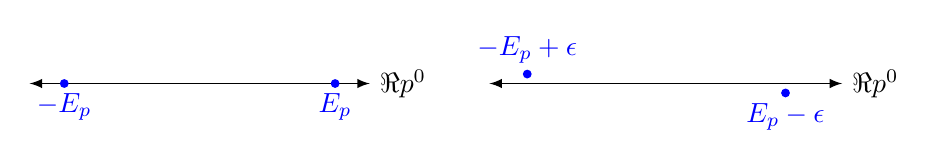
\begin{tikzpicture}[thick, scale=0.4]
    \draw[line width = 0.2mm, black, <->, >=latex] (-12.3,-2.6)--(-1.5,-2.6) node[right]{$\Re p^0$};
    \filldraw[blue](-11.2,-2.6)circle(2.9pt) node[below, blue] {$-E_p$};
    \filldraw[blue](-2.6,-2.6)circle(2.9pt) node[below, blue] {$E_p$};
    \draw[line width = 0.2mm, black, <->, >=latex] (2.3,-2.6)--(13.5,-2.6) node[right]{$\Re p^0$};
    \filldraw[blue](3.5,-2.3)circle(2.9pt) node[above, blue] {$-E_p+\ii \epsilon$};
    \filldraw[blue](11.7,-2.9)circle(2.9pt) node[below, blue] {$E_p-\ii \epsilon$};
    \end{tikzpicture}
    \caption{Cambio infinitesimal en la posición de los polos.}
    \label{fig_3.1}
\end{figure}

Cambiando infinitesimalmente la posición de los polos del eje real como se indica en la figura (\ref{fig_3.1}), es posible replantear la forma de $G(p)$ presente en la integral (\ref{eq_3.118}). Vamos a determinar dichos polos, entonces partimos de la prescripción propuesta por Feynman la cual modifica la ecuación (\ref{eq_3.117}) introduciendo un parámetro $\epsilon^\prime \to 0$,

\newcommand{\pf}{\Delta_F}
\begin{equation}
    \pf(p) = \frac{1}{p^2 - m^2 + \ii \epsilon^\prime},
    \label{eq_3.119}
\end{equation}
donde los ceros en el denominador (polos) se hallan de la siguiente manera:

\begin{prof}
	
	\begin{IEEEeqnarray*}{rCl}
		p^2-m^2 + \ii \epsilon^\prime &=& \qty(p^0)^2 - \qty( \vb*{p}^2+m^2 ) + \ii \epsilon^\prime = \qty(p^0)^2 - E_p^2 + \ii \epsilon^\prime = 0\\
		&& \implies \qty(p^0)^2 =  E_p^2 - \ii \epsilon^\prime\\
		&& \implies p^0 = \pm \sqrt{E_p^2 - \ii \epsilon^\prime} = \pm E_p \sqrt{1 - \ii \frac{\epsilon^\prime}{E_p^2}} \approx \pm E_p\qty( 1 - \frac{\epsilon^\prime}{2E_p^2}) ,
	\end{IEEEeqnarray*}
	
	de manera que ahora los polos de la integral (\ref{eq_3.118}) en $p^0$ están en el plano complejo en los puntos
	\begin{equation}
		p^0 = \pm (E_p - \ii \epsilon), \quad \quad  \epsilon \equiv \frac{\epsilon^\prime}{2E_p} 
	\end{equation}
	lo que nos permite escribir el denominador de (\ref{eq_3.119}) como
	
	\begin{equation*}
		\begin{split}
			\qty\big(p^0+\qty(E_p - \ii \epsilon))\qty\big(p^0 - \qty(E_p - \ii \epsilon)) &= \qty\big(\qty(p^0)^2 - \qty(E_p - \ii \epsilon)^2) \\
			&= \qty(p^0)^2 - E_p^2 + 2\ii E_p \epsilon + \underbrace{\epsilon^2}_{\approx 0}\\
			&= \qty(p^0)^2 - E_p^2  + \ii \epsilon^\prime.
		\end{split}
	\end{equation*}
	
	Hemos demostrado entonces que la ecuación (\ref{eq_3.119}) puede escribirse como
	
	\begin{equation}
		\begin{split}
			\pf (p) &= \frac{1}{\qty\big(p^0+\qty(E_p - \ii \epsilon))\qty\big(p^0-\qty(E_p - \ii \epsilon))}\\
			&=\frac{1}{2E_p} \qty[ \frac{1}{p^0-\qty(E_p - \ii \epsilon)} - \frac{1}{p^0+\qty(E_p - \ii \epsilon)} ] 
		\end{split}
	\end{equation}
	donde se ha expresado el resultado aplicando fracciones parciales. Con esto ya podemos replantear la integral (\ref{eq_3.118}) asociada a la función de Green $G\qty(x-x^\prime) \equiv \Delta_F \qty(x-x^\prime)$ como siendo
	
	\begin{IEEEeqnarray}{rCl}
		\pf \qty(x-x^\prime) &=& \int \frac{\dd[4]{p}}{\qty(2\pi)^4} \frac{\ee^{- \ii p(x-x^\prime)}}{ p^2 - m^2 + \ii \epsilon^\prime } \notag \\
		&=& \int \frac{\dd[4]{p}}{\qty(2\pi)^4} \frac{\ee^{- \ii p(x-x^\prime)}}{2E_p} \qty[ \frac{1}{p^0-\qty(E_p - \ii \epsilon)} - \frac{1}{p^0+\qty(E_p - \ii \epsilon)} ]\notag \\
		&=& \int \frac{\dd[3]{p}}{\qty(2\pi)^3} \frac{\ee^{ \ii \vb*{p}\cdot(\vb*{x}-\vb*{x}^\prime)}}{2E_p} \int_{-\infty}^{\infty} \frac{\dd{p^0}} {\qty(2\pi)} \qty[ \frac{\ee^{- \ii p^0(t-t^{\prime})}}{p^0-\qty(E_p - \ii \epsilon)} - \frac{\ee^{- \ii p^0(t-t^{\prime})}}{p^0+\qty(E_p - \ii \epsilon)} ].
		\label{eq_3.122}
	\end{IEEEeqnarray}
	
\end{prof}


Para evaluar la integral (\ref{eq_3.122}) en $p^0$, aplicamos variable compleja. Para ello vamos a resolver la siguiente integral.
    
    \begin{equation}
    	\boxed{
        \int_{-\infty}^\infty \frac{\ee^{-ia \zeta }}{\zeta+ib} \dd{\zeta} }\, .
        \label{eq_3.123}
    \end{equation}

Reescribimos la integral en el plano complejo y contemplemos dos casos.


\begin{itemize} 
    \item[$i)$] Si $a<0$, el exponente de la exponencial en la integral será negativo. Veamos que sucede con su parte real,
        \begin{equation}
            \Re \qty\big(-\ii a \zeta) = \Re \qty\big(-\ii a \qty(\zeta_x + \ii \zeta_y)) =  \Re \qty\big(-\ii a \zeta_x + \zeta_y) ) = a \zeta_y,
            \label{eq_3.124}
        \end{equation}
    indicándonos que $\Re \qty\big(-\ii a \zeta)$ es positiva si $\zeta_y < 0$ y negativa si $\zeta_y > 0$.   

    \begin{minipage}[b]{0.7\textwidth}
    Por lo tanto, para evaluar (\ref{eq_3.123}) es necesario que la parte real del exponente de la exponencial sea negativa, de modo que conviene trabajar con un contorno $c$ semicircular definido en la parte positiva de $\Im \zeta$, tal como se muestra en la figura (\ref{fig_3.2}).\\
    
    Antes de evaluar la integral, para evaluarlas aplicaremos el \emph{Teorema de residuos}, el cual establece
    \end{minipage}\hfill 
    \begin{minipage}[b]{0.3\textwidth}
        \begin{figure}[H]
        \centering
        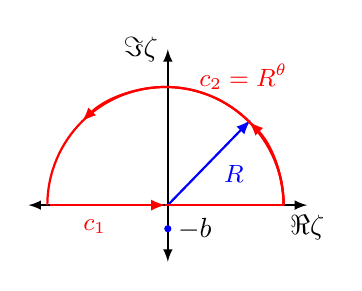
\begin{tikzpicture}[thick, scale=0.3]
            \node[below, red] at (6.8,3.8){\small $c_2 = R\ee^{\ii\theta}$};
            \node[below, red] at (0.5,-2.8){\small $c_1$};
            \node[below, blue] at (6.4,-0.5){\small{$R$}};
            \draw[line width = 0.2mm, black, <->, >=latex] (-2.3,-2.6)--(9.5,-2.6) node[below]{$\Re \zeta$};
            \draw[line width = 0.2mm, black, <->, >=latex] (3.6,-5)--(3.6,4.0) node[left]{$\Im \zeta$};
            \draw[red, ->, >=latex ](-1.4,-2.6) -- (3.5,-2.6);
            \draw[blue, ->, >=latex ](3.6,-2.6) -- (7.1,1.0);
            \draw[red](3.5,-2.6) -- (8.5,-2.6);
            \draw[red] (8.5,-2.6) arc (0:180:5);
            \draw[red, ->, >=latex] (8.5,-2.6) arc (0:45:5);
            \draw[red, ->, >=latex] (8.5,-2.6) arc (0:135:5);
            \filldraw[blue](3.6,-3.6)circle(2.9pt) node[right, black] {$-\ii b$};
        \end{tikzpicture}
        \caption{\small{Curva $c$.}}
        \label{fig_3.2}
        \end{figure}
    \end{minipage}

    \begin{theorem} [Teorema de la curva de Cauchy]
        Si $f(z)$ es una función holomorfa, la integral sobre un contorno $c$ (no importa la forma) que encierra un punto singular $z_0$ es
            \begin{equation}
                \oint_{c} f(z) dz = 2\pi \ii \Res_{z_0} \qty(f(z)), 
            \end{equation} 
        siendo $\Res_{z_0}(f(z))$, el residuo de la función en el punto $z_0$. Si $z_0$ es un polo de orden $n$, la expresión para calcular el residuo es 
            \begin{equation}
                \Res_{z_0}(f(z))=\frac{1}{(n-1)!} \lim_{z\to z_0} \frac{d^{n-1}}{dz^{n-1}}\qty\big(\qty(z-z_0)^n f(z)).
            \end{equation}
        Si el contorno no encierra ninguna singularidad, la integral sobre este es cero.
    \end{theorem}

    Entonces podemos escribir la integral (\ref{eq_3.123}) como

    \begin{equation}
        \oint_{c} \frac{\ee^{-\ii a \zeta}}{z+\ii b} \dd{\zeta} = \int_{c_1} \frac{\ee^{-\ii a \zeta}}{\zeta+\ii b} \dd{\zeta} + \int_{c_2} \frac{\ee^{-\ii a \zeta}}{\zeta+\ii b} \dd{\zeta} = 0.
        \label{eq_3.127}
    \end{equation}
    Al evaluar la integral sobre $c_2$,
    \begin{equation*}
        \begin{split}
            \int_{c_2}  \frac{\ee^{-\ii a \zeta}}{z+\ii b} \dd{\zeta} &= \ii \lim_{R \to \infty} \int_0^\pi \dd{\theta} R\ee^{\ii \theta} \frac{\ee^{-\ii a R \ee^{\ii \theta}}}{R \ee^{\ii \theta}+\ii b} \approx \ii \lim_{R \to \infty} \int_0^\pi \dd{\theta} R\ee^{\ii \theta} \frac{\ee^{-\ii a R \ee^{\ii \theta}}}{R \ee^{\ii \theta}} \\
            &= \ii \lim_{R \to \infty} \int_0^\pi \dd{\theta} \ee^{-\ii a R \cos \theta }\ee^{a R \sin \theta } \to 0, 
        \end{split}
    \end{equation*}
    donde se ha considerado el hecho que $a<0$ en el límite cuando $R\to \infty$ para el termino $\ee^{a R \sin \theta }$, además la cantidad $\ee^{-ia R \cos \theta }$ siempre será acotada aun cuando consideremos el límite al infinito.\\

    Entonces, la integral (\ref{eq_3.127}) se reduce solo sobre el eje real ($c_1$) y resulta
    \begin{equation}
        \int_{-\infty}^\infty \frac{\ee^{-\ii a \zeta}}{\zeta+\ii b} \dd{\zeta} = 0.
        \label{eq_3.128}
    \end{equation} 
    
    \begin{minipage}[b]{0.7\textwidth}
    \item[$ii)$] Si $a>0$, la ecuación (\ref{eq_3.124}) nos indica que $\Re \qty\big(-\ii a \zeta)$ es positiva si $\zeta_y > 0$ y negativa si $\zeta_y < 0$.\\
    
    En consecuencia, conviene trabajar con un contorno semicircular definido en la parte negativa del eje imaginario $\Im \zeta$ como se muestra en la figura (\ref{fig_3.3}). Así se garantizará que la integral sobre el arco $c_2$ al tomar el límite al infinito, decaiga a cero.\\
    \end{minipage}\hfill 
    \begin{minipage}[b]{0.3\textwidth}
        \begin{figure}[H]
        \centering
        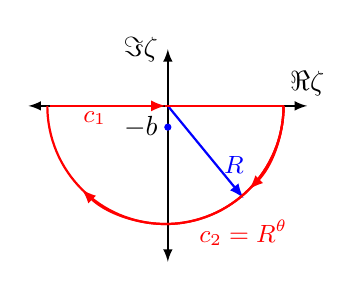
\begin{tikzpicture}[thick, scale=0.3]
            \node[below, red] at (6.8,-2.8){\small $c_2 = R\ee^{\ii\theta}$};
            \node[below, red] at (0.5,1.8){\small $c_1$};
            \node[below, blue] at (6.4,-0.1){\small{$R$}};
            \draw[line width = 0.2mm, black, <->, >=latex] (-2.3,1.6)--(9.5,1.6) node[above]{$\Re \zeta$};
            \draw[line width = 0.2mm, black, <->, >=latex] (3.6,-5)--(3.6,4.0) node[left]{$\Im \zeta$};
            \draw[red, ->, >=latex ](-1.4,1.6) -- (3.5,1.6);
            \draw[blue, ->, >=latex ](3.6,1.6) -- (6.8,-2.3);
            \draw[red](3.5,1.6) -- (8.5,1.6);
            \draw[red] (8.5,1.6) arc (0:-180:5);
            \draw[red, ->, >=latex] (8.5,1.6) arc (0:-45:5);
            \draw[red, ->, >=latex] (8.5,1.6) arc (0:-135:5);
            \filldraw[blue](3.6,0.7)circle(2.9pt) node[left, black] {$-\ii b$};
        \end{tikzpicture}
        \caption{\small{Curva $c$.}}
        \label{fig_3.3}
        \end{figure}
    \end{minipage}   

    Así,

    \begin{equation}
        \oint_c \frac{\ee^{-\ii a \zeta}}{\zeta+\ii b} \dd{\zeta} = \int_{c_1} \frac{\ee^{-\ii a \zeta}}{\zeta+\ii b} \dd{\zeta} + \int_{c_2} \frac{\ee^{-\ii a \zeta}}{\zeta+\ii b} \dd{\zeta} = - 2\pi \ii \Res_{-\ii b} \qty(\frac{\ee^{-\ii a \zeta}}{\zeta+\ii b}),
        \label{eq_3.129}
    \end{equation}
    donde el signo menos en el resultado se debe a que recorremos la trayectoria en sentido horario. El residuo de la función es 
    \begin{equation}
        \Res_{-ib} \qty(\frac{\ee^{-\ii a \zeta}}{\zeta+\ii b})=\lim_{ \zeta \to -\ii b} \cancel{\qty( \zeta + \ii b)}\frac{\ee^{-\ii a \zeta}}{\cancel{\qty(\zeta+\ii b)}} = \ee^{-ab},
    \end{equation}
    además nuevamente en el límite cuando $R\to \infty$ se tiene que 
    \begin{equation*}
        \begin{split}
            \int_{c_2} \frac{\ee^{-\ii a \zeta}}{\zeta+\ii b} \dd{\zeta} & \approx \ii \lim_{R \to \infty} \int_{2\pi}^{\pi}  \dd{\theta} R\ee^{\ii \theta} \frac{\ee^{-\ii a R \ee^{\ii \theta}}}{R \ee^{\ii \theta}}\\
            &= \ii \lim_{R \to \infty} \int_{2\pi}^{\pi}  \dd{\theta} \ee^{-\ii a R\cos \theta}\ee^{a R\sin  \theta}\to 0, 
        \end{split}
    \end{equation*}
    la cual tiende a cero por el término $\ee^{a R\sin  \theta}$ con $R\to \infty$, debido a que $\sin \theta$ es negativo en el intervalo de integración. La expresión $\ee^{-\ii a R\cos \theta}$ no afecta en el límite porque nuevamente permanece acotada en el límite. Así en (\ref{eq_3.129}) en el límite de $R$ al infinito, la integral sobre $c_1$ es

    \begin{equation}
        \int_{-\infty}^\infty \frac{\ee^{-\ii a \zeta}}{\zeta+\ii b} \dd{\zeta} = - 2\pi \ii \ee^{-ab}.
        \label{eq_3.131}
    \end{equation}
\end{itemize}
Vamos a considerar $b=\epsilon \to 0$, en la integral (\ref{eq_3.123}) pues nos será mas conveniente de esa manera. Entonces las soluciones (\ref{eq_3.128}) y (\ref{eq_3.131}) son

\begin{IEEEeqnarray*}{rCl}
    a<0 & \implies & \int_{-\infty}^\infty \frac{\ee^{-\ii a \zeta}}{\zeta+\ii \epsilon} \dd{\zeta} = 0\\
    a>0 & \implies & \int_{-\infty}^\infty \frac{\ee^{-\ii a \zeta}}{\zeta+\ii \epsilon} \dd{\zeta} = - 2\pi \ii, 
\end{IEEEeqnarray*}

que lo podemos escribir usando la función Heaviside de la forma

\begin{equation}
    \boxed{
    \int_{-\infty}^\infty  \frac{\ee^{-\ii a \zeta}}{\zeta+\ii \epsilon} \dd{\zeta}= - 2\pi \ii \Theta(a) } \, .
    \label{eq_3.132}
\end{equation}

Con este resultado, podemos evaluar cada una de las integrales de la ecuación (\ref{eq_3.122}). Comencemos con

\begin{equation*}
    I_1 \equiv \int_{-\infty}^\infty \frac{\dd{p^0}} {\qty(2\pi)} \frac{\ee^{ -\ii p^0(t-t^{\prime})}}{\qty\big(p^0-\qty(E_p - \ii \epsilon))},
\end{equation*}
la cual podemos reescribir haciendo\footnote{Las variables $p^0$ y $E_p$ no son las mismas, dado que al inicio de la sección se propuso que cada una de las componentes del cuadrivector $p^\mu$ sean independientes entre si} $p^{0 \prime}=p^0-E_p$ de modo que $dp^{0 \prime}=dp^0$, por lo tanto

\begin{IEEEeqnarray}{rCl}
    I_1 = \int_{-\infty}^\infty \frac{\dd{p^{0 \prime}}} {\qty(2\pi)} \frac{\ee^{- \ii \qty(p^{0\prime}+E_p)(t-t^{\prime})}}{\qty( p^{0 \prime} + \ii \epsilon)} &=& \ee^{- \ii E_p(t-t^{\prime})} \int_{-\infty}^\infty \frac{\dd{p^{0 \prime}}} {\qty(2\pi)} \frac{\ee^{- \ii p^{0\prime}(t-t^{\prime})}}{\qty( p^{0 \prime} + \ii \epsilon)} \notag \\
    &=&- \ii \Theta(t-t^{\prime}) \ee^{- \ii E_p(t-t^{\prime})} ,
    \label{eq_3.133}
\end{IEEEeqnarray}
donde se ha usado (\ref{eq_3.132}). Ahora evaluamos

\begin{equation*}
    I_2 \equiv \int_{-\infty}^\infty \frac{\dd{p^0}} {\qty(2\pi)} \frac{\ee^{ -\ii p^0(t-t^{\prime})}}{\qty\big(p^0+\qty(E_p - \ii \epsilon))},
\end{equation*}
donde se considera $p^{0 \prime}=-\qty(p^0+E_p)$ de modo que $dp^{0 \prime}=-dp^0$, así

\begin{IEEEeqnarray}{rCl}
    I_2 = - \int_{\infty}^{-\infty} \frac{\dd{p^{0 \prime}}} {\qty(2\pi)} \frac{\ee^{ -\ii \qty(-p^{0\prime} - E_p)(t-t^{\prime})}}{\qty( -p^{0 \prime} - \ii \epsilon)} &=& - \ee^{- \ii E_p(t^{\prime}-t)} \int_{-\infty}^\infty \frac{\dd{p^{0 \prime}}} {\qty(2\pi)} \frac{\ee^{-\ii p^{0\prime}(t^{\prime}-t)}}{\qty(p^{0 \prime} + \ii \epsilon)} \notag \\
    &=& \ii \Theta(t^{\prime}-t) \ee^{- \ii E_p(t^{\prime}-t)} .
    \label{eq_3.134}
\end{IEEEeqnarray}

Empleando (\ref{eq_3.133}) y (\ref{eq_3.134}) en el propagador (\ref{eq_3.122}),

\begin{IEEEeqnarray}{rCl}
    \pf \qty(x-x^\prime) &=& - \ii \int \frac{\dd[3]{p}}{\qty(2\pi)^3} \frac{\ee^{ \ii \vb*{p}\cdot(\vb*{x}-\vb*{x}^\prime)}}{2E_p} \qty[ \Theta(t-t^{\prime}) \ee^{- \ii E_p(t-t^{\prime})} + \Theta(t^{\prime}-t) \ee^{- \ii E_p(t^{\prime}-t)}] \notag \\
    \pf \qty(x-x^\prime) &=& - \ii \int \frac{\dd[3]{p}}{2E_p \qty(2\pi)^3} \qty[ \Theta(t-t^{\prime}) \ee^{ - \ii E_p(t-t^{\prime}) + \ii \vb*{p}\cdot(\vb*{x}-\vb*{x}^\prime)} + \Theta(t^{\prime}-t) \ee^{- \ii E_p(t^{\prime}-t)+\ii \vb*{p}\cdot(\vb*{x}-\vb*{x}^\prime)} ]. $\IEEEeqnarraynumspace$
    \label{eq_3.135}
\end{IEEEeqnarray}

Al hacer el cambio de variable $ \vb*{p^\prime}\to \vb*{-p}$ en la segunda integral,

\begin{IEEEeqnarray*}{rCl}
    $\faDribbble$ & \equiv & \int \frac{\dd[3]{p}}{2E_p \qty(2\pi)^3} \Theta(t^{\prime}-t) \ee^{- \ii E_p(t^{\prime}-t)+\ii \vb*{p}\cdot(\vb*{x}-\vb*{x}^\prime)} \\ 
    &=& (-1)^3 \int_{\infty}^{-\infty} \frac{\dd[3]{p^\prime}}{2E_{-p^\prime}} \Theta(t^{\prime}-t) \ee^{- \ii E_{-p^\prime}(t^{\prime}-t)-\ii \vb*{p}^\prime \cdot(\vb*{x}-\vb*{x}^\prime)} ,
\end{IEEEeqnarray*}
donde ya se demostró que $E_{-p}=E_p$ y los límites en las tres integrales se reajustan por el factor $(-1)^3$. Entonces cambiamos nuevamente la variable de integración $\vb*{p}^\prime \to \vb*{p}$

\begin{IEEEeqnarray}{rCl}
    $\faDribbble$ &=& \int \frac{\dd[3]{p}}{2E_{p}} \Theta(t^{\prime}-t) \ee^{\ii E_{p}(t-t^{\prime})-\ii \vb*{p}\cdot(\vb*{x}-\vb*{x}^\prime)}.
\end{IEEEeqnarray}
Con lo anterior reescribimos el propagador de Feynman (\ref{eq_3.135}),

\begin{IEEEeqnarray}{rCl}
    \ii \pf \qty(x-x^\prime) &=& \int \frac{\dd[3]{p}}{2E_p \qty(2\pi)^3} \qty[ \Theta(t-t^{\prime}) \ee^{ - \ii E_p(t-t^{\prime}) + \ii \vb*{p}\cdot(\vb*{x}-\vb*{x}^\prime)} + \Theta(t^{\prime}-t) \ee^{ \ii E_p(t-t^{\prime})-\ii \vb*{p}\cdot(\vb*{x}-\vb*{x}^\prime)} ] , \notag 
\end{IEEEeqnarray}

\begin{equation}
    \boxed{\ii \pf \qty(x-x^\prime)  = \int \frac{\dd[3]{p}}{2E_p \qty(2\pi)^3} \qty[ \Theta(t-t^{\prime}) \ee^{-\ii p(x-x^{\prime})} + \Theta(t^{\prime}-t) \ee^{\ii p(x-x^{\prime})} ] } \, .
    \label{eq_3.137}
\end{equation}

siendo ahora \emph{las componentes del cuadrivector} $p \equiv (E_p,\vb*{p})$ con $E_p=\sqrt{\vb*{p}^2+m^2}$.\\

Como ejercicio se deja demostrar que el propagador de Feynman satisface la ecuación que define la función de Green (\ref{eq_3.107})

\begin{equation}
    \qty(\square_x + m^2)\pf(x-x^\prime)=-\delta^4 (x-x^\prime). 
\end{equation}
garantizando el hecho de que es una \emph{función de Green} de la ecuación de movimiento.\\

Una ves estudiado el propagador de Feynman como una función de Green, miremos como se relaciona con la cuantización de los campos. Si analizamos solamente el campo escalar real, 

\begin{equation*}
    \Ophi \left(x\right) =  \int \frac{\dd[3]{p}}{\sqrt{2\qty(2\pi)^{3}E_p}} \qty\bigg[\Oa_p \ee^{-\ii px} + \Oa^{\dag}_p\ee^{\ii px}].
\end{equation*}

La acción de este operador sobre el estado \emph{vacio} junto con las expresiones (\ref{eq_3.57}) y (\ref{eq_3.67}) implican

\begin{IEEEeqnarray}{rCl}
    \Ophi \left(x\right) \ket{0} &=& \int \frac{\dd[3]{p}}{\sqrt{2\qty(2\pi)^{3}E_p}} \qty\bigg[ \cancelto{0}{\Oa_p \ket{0}}\ee^{-\ii px} + \Oa^{\dag}_p \ket{0} \ee^{\ii px}] \notag \\
    &=& \int \frac{\dd[3]{p}}{\sqrt{2\qty(2\pi)^{3}E_p}} \ee^{\ii px} \ket{p}.
    \label{eq_3.139}
\end{IEEEeqnarray}

Al tomar el adjunto hermítico de $\ket{p} = \Oa^\dag_p \ket{0}$, demostramos que era de la forma $\bra{p}=\bra{0}\Oa_p$. Calculando la acción del campo escalar real sobre el $\bra{0}$,

\begin{IEEEeqnarray}{rCl}
    \bra{0}\Ophi \qty(x^\prime) &=& \int \frac{\dd[3]{p^\prime}}{\sqrt{2\qty(2\pi)^{3}E_{p^\prime}}} \qty\bigg[  \bra{0}\Oa_{p^\prime} \ee^{-\ii p^\prime x^\prime} + \cancelto{0}{\bra{0} \Oa^{\dag}_{p^\prime}}\ee^{\ii p^\prime x^\prime}]\notag \\
    &=& \int \frac{\dd[3]{p^\prime}}{\sqrt{2\qty(2\pi)^{3}E_{p^\prime}}} \ee^{-\ii p^\prime x^\prime} \bra{p^\prime}.
    \label{eq_3.140}
\end{IEEEeqnarray}

Los resultados anteriores nos permiten calcular dos cosas. Lo primero es que el valor esperado del campo escalar real en el estado vacío es cero, puesto que

\begin{equation}
    \ev{\Ophi \qty(x)}{0} = \int \frac{\dd[3]{p}}{\sqrt{2\qty(2\pi)^{3}E_p}} \ee^{\ii px} \cancelto{0}{\braket{0}{p}} = 0.
\end{equation}

Y la segunda, que el valor esperado del operador $\Ophi$ elevado al cuadrado es diferente de cero. Es decir

\begin{IEEEeqnarray}{rCl}
    \ev{ \Ophi \qty(x^\prime) \Ophi \qty(x)}{0} &=& \qty(\int \frac{\dd[3]{p^\prime}}{\sqrt{2\qty(2\pi)^{3}E_{p^\prime}}} \ee^{-\ii p^\prime x^\prime} \bra{p^\prime}) \qty( \int \frac{\dd[3]{p}}{\sqrt{2\qty(2\pi)^{3}E_p}} \ee^{\ii px} \ket{p} ) \notag \\
    &=& \int \int \frac{\dd[3]{p^\prime}}{\sqrt{2\qty(2\pi)^{3}E_{p^\prime}}} \frac{\dd[3]{p}}{\sqrt{2\qty(2\pi)^{3}E_p}} \ee^{\ii \qty( px - p^\prime x^\prime) } \underbrace{\braket{p^\prime}{p}}{\delta^3(\vb*{p}^\prime-\vb*{p}) }  \, . \notag 
\end{IEEEeqnarray}

\begin{equation}
    \boxed{
    \ev{ \Ophi \qty(x^\prime) \Ophi \qty(x)}{0} = \int  \frac{\dd[3]{p}}{2\qty(2\pi)^{3}E_p} \ee^{\ii p \qty(x - x^\prime)} } \, .
    \label{eq_3.142}
\end{equation}
Análogamente podemos calcular

\begin{equation}
    \boxed{
    \ev{ \Ophi \qty(x) \Ophi \qty(x^\prime)}{0} = \int  \frac{\dd[3]{p}}{2\qty(2\pi)^{3}E_p} \ee^{\ii p \qty(x^\prime - x)} } \, .
    \label{eq_3.143}
\end{equation}

Note que en la ultima expresión si hacemos el cambio e variable $ \vb*{p} \to -\vb*{p}$, no tenemos problema con el diferencial y los limites de integración, pero el exponente se transforma en

\begin{equation*}
    p(x^\prime-x) = p_0(x^{0\prime} - x^0 ) - \vb*{p}(\vb*{x^\prime}-\vb*{x}) \quad \to \quad  p_0(x^0 - x^{0\prime}) + \vb*{p}(\vb*{x^\prime}-\vb*{x}),
\end{equation*}

es decir el exponente de las expresiones (\ref{eq_3.142}) y (\ref{eq_3.143}) no son iguales, no quedan en forma covariante y por lo tanto

\begin{equation}
    \boxed{
    \ev{ \Ophi \qty(x^\prime) \Ophi \qty(x)}{0} \neq  \ev{ \Ophi \qty(x) \Ophi \qty(x^\prime)}{0} } \, .
\end{equation}

Ahora vamos a emplear el propagador (\ref{eq_3.137}), para escribirlo en términos de los operadores de campo $\Ophi$. Reemplacemos cada una de las integrales de (\ref{eq_3.137}) por su equivalente en términos de operadores (\ref{eq_3.142}) y (\ref{eq_3.143}),

\begin{equation}
    \boxed{
    \ii \pf \qty(x-x^\prime)  = \Theta(t-t^{\prime}) \ev{ \Ophi \qty(x) \Ophi \qty(x^\prime)}{0} + \Theta(t^{\prime}-t) \ev{ \Ophi \qty(x^\prime) \Ophi \qty(x)}{0} } \, .
    \label{eq_3.145}
\end{equation}

es decir como una suma pesada de dos funciones de dos puntos. Es mas usual expresar el propagador en términos del \emph{operador de ordenamiento temporal}, es decir

\newcommand{\OrdT}{\mathcal{T}}

\begin{equation}
    \boxed{\ii \pf \qty(x-x^\prime)  = \ev{ \OrdT \qty\big[ \Ophi \qty(x) \Ophi \qty(x^\prime) ]}{0} } \, .
\end{equation}

donde $\OrdT$ para campos bosónicos está definido como

\begin{equation}
    \boxed{
    \OrdT \qty\big[ A \qty(x) B \qty(x^\prime) ] = \left\{ \,
    \begin{IEEEeqnarraybox}[][c]{l?s}
        \IEEEstrut
            A \qty(x) B \qty(x^\prime) & Si $\quad t>t^\prime$  \\
            B \qty(x^\prime) A \qty(x) & Si $\quad t<t^\prime$ 
        \IEEEstrut
    \end{IEEEeqnarraybox}
    \right.
    \label{eq_3.147}} \, .
\end{equation}

El operador $\OrdT \qty [ ... ]$ representa un producto de operadores ordenados por el tiempo, donde el operador con el tiempo posterior debe colocarse a la izquierda del operador con el tiempo anterior.\\

Interpretemos (\ref{eq_3.145}). Si $t<t^{\prime}$, solo sobrevive el segundo término asociado a $\ev{ \Ophi \qty(x^\prime) \Ophi \qty(x)}{0}$. Para entenderlo, recordemos que de (\ref{eq_3.139}) el operador $\Ophi(x)$ actuando sobre el \emph{vacío} crea una \emph{partícula} en el tiempo $t$ y con momento $\vb*{p}$. Pero, la acción del operador $\Ophi(x^\prime)$ sobre el $\bra{0}$ en (\ref{eq_3.140}) se caracteriza porque solo contribuye la parte asociada al operador destrucción, y por tanto lo podemos interpretar como la destrucción de una partícula en un tiempo $t^\prime$. En conclusión el elemento de matriz $\ev{ \Ophi \qty(x^\prime) \Ophi \qty(x)}{0}$ describe la \emph{amplitud de una partícula} que se crea en el tiempo $t$, se propaga en el espacio-tiempo y se destruye en un tiempo posterior $t^\prime$.\\

De la misma manera, si $t > t^\prime $ solo sobrevive el primer término de (\ref{eq_3.145}) asociado al elemento de matriz $\ev{ \Ophi \qty(x) \Ophi \qty(x^\prime)}{0}$, el cual describe la amplitud de una partícula que se crea en el tiempo $t^\prime$, se propaga en el espacio tiempo y se destruye en el tiempo posterior $t$. Esto es el sentido físico del propagador, elemento importante para calcular las amplitudes de varios procesos que involucran interacciones de partículas.

\section{Adicional: Interpretación de partícula y función de n Puntos}

\subsection{Interpretación de Partícula}

En la sección \ref{Efockes} comentamos que los estados construidos a partir de actuar con $n$ operadores de creación sobre el vacío podían considerarse como estados de $n$ partículas con momentos definidos (\emph{multipartículas}). Vamos a ver, siguiendo un ejercicio, que los estados dados por $\Ophi(t,\vb*{x})\ket{0} $ describen lo más cercano que uno puede tener a la noción de partícula localizada en un punto del espacio $\vb*{x}$ a tiempo $t$.\\

Vamos a analizar en qué medida la teoría del campo escalar real libre, restringida a los estados de una partícula, puede ser considerada como una generalización relativista de la teoría de Schrödinger, y como el operador $\Ophi(x)$ puede ser asimilado a un operador de creación de una partícula en un punto del espacio. Primero vamos a mostrar que los vectores $\Ophi(x)=\Ophi(t,\vb*{x})$ a un tiempo fijo generan todo el espacio de Hilbert $\mathscr{H}_1$ de una partícula.\\

Para simplificar el desarrollo, tomamos el tiempo fijo $t=0$ (el resultado no cambia). Lo que se pretende ver en este inciso es que haciendo combinaciones lineales de los estados dados por $\hat{\phi}(0, \vb*{x})\ket{0}$ podemos generarnos un estado de una partícula con una distribución arbitraria de momentos. Es decir, queremos ver que podemos fabricarnos un estado de la forma

\begin{equation}
    \int \frac{\dd[3]{p}}{\sqrt{2E_p(2 \pi)^3}} c(\vb*{p})\ket{\vb*{p}},
    \label{eq_3.148}
\end{equation}

donde $\ket{\vb*{p}} \equiv \hat{a}_{\vb*{p}}^{\dagger}|0\rangle$ y $c(\vb*{p})$ es una función arbitraria (que es la que determina la distribución de momentos del estado). Mantuvimos el factor $\sqrt{2 (2 \pi)^{3} {E_p}}$ al hacer la combinación lineal, pero podrían absorberse en la definición de $c(\vb*{p})$ (lo que importa es que estamos haciendo una combinación lineal).\\

Veamos qué forma tiene el estado $\hat{\phi}(0,\vb*{x})\ket{0}$. Recordando la expresión (\ref{eq_3.139}) para $t=0$, tenemos

\begin{equation}
    \hat{\phi}(0, \vb*{x})|0\rangle=\int \frac{\dd[3]{p}}{ \sqrt{2 (2 \pi)^{3} E_p}} \ee^{-\ii \vb*{p} \cdot \vb*{x}}\ket{\vb*{p}}.
\end{equation}

Ya que $\hat{a}_{p}\ket{0}=0$ y $\hat{a}_{p}^{\dagger}\ket{0}=\ket{\vb*{p}}$. Una combinación lineal arbitraria de estos estados, con coeficientes $f(\vb*{x})$, tendrá entonces la forma

\begin{equation}
    \int \dd[3]{x} f(\vb*{x}) \Ophi(0,\vb*{x})\ket{0} = \int \frac{\dd[3]{p}}{\sqrt{2\qty(2\pi)^3 E_p}}\qty[\int \dd[3]{x} f(\vb*{x})\ee^{-\ii \vb*{p} \cdot \vb*{x}}] \ket{\vb*{p}},
    \label{eq_3.150}
\end{equation}

Para conseguir un estado de la forma (\ref{eq_3.148}) necesitamos que el término entre corchetes en (\ref{eq_3.150}) sea igual a $c(\vb*{p})$. Esto se puede conseguir sencillamente tomando a $c(\vb*{p})$ como la transformada de Fourier de $f(\vb*{x})$.

Vimos entonces que una combinación lineal de estados $\hat{\phi}(0, \vb*{x})\ket{0}$ generan el espacio de Hilbert $\mathscr{H}_1$ asociado a una partícula en  un tiempo fijo $t$ .\\

Se define el estado $\ket{t,\vb*{x}}$ (\emph{Supuestos vectores de una partícula localizados}) y la función de onda $\psi \qty(t,\vb*{x}) \equiv \braket{t,\vb*{x}}{\psi}$, con $\ket{\psi} \in \mathscr{H}_1$ (\emph{Supuesta función de onda correspondiente a una partícula}). Vamos a probar que $\psi \qty(t,\vb*{x})$ satisface la ecuación KG. Además se demostrará que satisface la ecuación diferencial de primer orden en derivadas temporales

\begin{IEEEeqnarray}{rCl}
	\ii \pdv{\psi (t,\vb*{x})}{t} = + \sqrt{m^2 - \laplacian } \psi(t,\vb*{x}),
	\label{eq_3.151}
\end{IEEEeqnarray}

Para demostrar que satisface la ecuación de Klein-Gordon es sencillo ya que el mismo campo $\Ophi$ la satisface, en efecto

\newcommand{\OKG}{\qty( \square + m^2 )}

\begin{IEEEeqnarray}{rCl}
	\OKG \psi(t,\vb*{x}) & = & \OKG	 \braket{t,\vb*{x}}{\psi} \notag \\
	&=& \OKG \bra{0} \Ophi(t,\vb*{x}) \ket{\psi} \notag \\
	&=& \bra{0} \OKG  \Ophi(t,\vb*{x}) \ket{\psi} = 0,
\end{IEEEeqnarray}

donde usamos que el campo es real (y por lo tanto es igual a su conjugado) y que cumple la ecuación de Klein-Gordon (\ref{eq_3.6}).

Adicionalmente vamos a demostrar que $\psi(t,\vb*{x})$ evoluciona solo con frecuencias positivas, es decir como el operador $\Oa_p$.  Esto también es sencillo  ver, ya que los operadores $\Oa^\dag_p$ aniquilan al vacío al actuar a la izquierda.

\begin{IEEEeqnarray}{rCl}
	\psi\qty(t,\vb*{x}) &=& \braket{t,\vb*{x}}{\psi} = \bra{0} \Ophi\qty(t,\vb*{x}) \ket{\psi} \notag \\
	& = &  \int \frac{\dd[3]{p}}{\sqrt{2\qty(2\pi)^{3}E_p}} \bra{0} \qty\bigg[\Oa_p \ee^{-\ii E_p t}\ee^{\ii \vb*{p} \cdot \vb*{x}} + \Oa^{\dag}_p\ee^{\ii E_p t}\ee^{-\ii \vb*{p} \cdot \vb*{x}}] \ket{\psi} \notag \\
	& = &  \int \frac{\dd[3]{p}}{\sqrt{2\qty(2\pi)^{3}E_p}}  \ee^{\ii \vb*{p} \cdot \vb*{x}} \bra{0} \Oa_p \ket{\psi} \ee^{-\ii E_p t},
\end{IEEEeqnarray}

noten que el operador $\sqrt{m^2 - \laplacian}$ esta bien definido ya que $\qty(m^2-\laplacian)$ es positivo, hecho que se puede ver calculando 

\begin{equation}
	\qty(m^2-\laplacian ) \psi(t,\vb*{x}) =   \qty(m^2 + \vb*{p}^2) \psi(t,\vb*{x})  = E_p^2 \psi(t,\vb*{x})~.
	\label{eq_3.154}
\end{equation}

Por otro lado, para ver que se cumple la ecuación (\ref{eq_3.151}) calculemos

\begin{equation}
	\ii \pdv{\psi (t,\vb*{x})}{t} = \ii \pdv{t} \int \frac{\dd[3]{p}}{\sqrt{2\qty(2\pi)^{3}E_p}}  \ee^{\ii \vb*{p} \cdot \vb*{x}} \bra{0} \Oa_p \ket{\psi} \ee^{-\ii E_p t} = E_p \psi (t,\vb*{x}),
\end{equation}
 
 y de (\ref{eq_3.154}) resulta que
 
  
 \begin{equation}
 	\ii \pdv{\psi (t,\vb*{x})}{t} = + \sqrt{m^2 - \laplacian } \psi (t,\vb*{x}). 
 \end{equation}
 
 Se deja a modo de ejercicio verificar que la corriente conservada de Klein-Gordon da lugar a una probabilidad conservada y positiva, pero la densidad de probabilidad no es definida positiva.\\
 
 Ahora, vamos a mostrar que el valor de $\braket{x}{y} \equiv \braket{t,\vb*{x}}{t,\vb*{y}}$ no es proporcional a la función delta de Dirac y que los estados $\ket{t,\vb*{x}}$ están localizados en un tamaño típico $\Delta x \thicksim 1/m $ (\emph{en unidades naturales corresponde a la Longitud de Compton} $\frac{\hbar}{mc} $ ).\\
 
 Si bien es cierto, en mecánica cuántica no relativista, los estados de una partícula localizada en puntos distintos del espacio son ortonormales, sin embargo, aquí no ocurre eso para los estados $\ket{x}$. Calculemos
 
 \begin{IEEEeqnarray}{rCl}
 	\braket{t,\vb*{x}}{t,\vb*{y}} & = & \ev{\Ophi(t,\vb*{x})\Ophi(t,\vb*{y})}{0} \notag \\
 	& = &  \int \frac{\dd[3]{p}}{\sqrt{2\qty(2\pi)^{3}E_p}} \int \frac{\dd[3]{p^\prime}}{\sqrt{2\qty(2\pi)^{3}E_{p^\prime}}} \ee^{-\ii \qty( E_p - E_p^{\prime}) t}\ee^{\ii \qty(\vb*{p} \cdot \vb*{x} - \vb*{p}^\prime \cdot \vb*{y} )}  \ev{\Oa_p \Oa_{p^\prime}^\dag}{0}  \notag \\
 	& = &  \int \frac{\dd[3]{p}}{\sqrt{2\qty(2\pi)^{3}E_p}} \int \frac{\dd[3]{p^\prime}}{\sqrt{2\qty(2\pi)^{3}E_{p^\prime}}} \ee^{-\ii \qty( E_p - E_p^{\prime}) t}\ee^{\ii \qty(\vb*{p} \cdot \vb*{x} - \vb*{p}^\prime \cdot \vb*{y} )} \delta^3 \qty(\vb*{p}-\vb*{p}^\prime) \notag \\
 	& = & \int \frac{\dd[3]{p}}{2\qty(2\pi)^{3}E_p} \ee^{\ii \vb*{p} \cdot  \qty( \vb*{x}  - \vb*{y} )} = \int \frac{\dd[3]{p}}{2\qty(2\pi)^{3}}  \frac{\ee^{\ii \vb*{p} \cdot  \qty( \vb*{x}  - \vb*{y} )} }{(\vb*{p}^2+m^2)}.
 \end{IEEEeqnarray}
 
 Para evaluar esta integral empleamos coordenadas esféricas $\qty(p,\varphi,\theta )$ considerando el ángulo azimutal $\theta$ como el ángulo entre los vectores $\vb*{p}$ y $(\vb*{x}-\vb*{y})$. Definiendo $u \equiv \abs{\vb*{x}-\vb*{y}}$,
 
 \begin{IEEEeqnarray*}{rCl}
 	\braket{t,\vb*{x}}{t,\vb*{y}} & = & \frac{1}{2 \qty(2\pi)^3} \int_{0}^{+\infty} \dd{p} p^2  \int_{0}^{2\pi} \dd{\varphi}  \int_{-1}^{1} \dd{(\cos \theta)} \frac{\ee^{\ii p u \cos \theta}}{\sqrt{p^2 + m^2}} \\
 	& = & \frac{1}{2 \qty(2\pi)^2} \int_{0}^{+\infty} \dd{p}  \frac{p^2}{\sqrt{p^2 + m^2}}  \int_{-1}^{1} \dd{(\cos \theta)} \ee^{\ii p u \cos \theta}\\
 	& = & \frac{1}{2 \qty(2\pi)^2} \int_{0}^{+\infty} \dd{p}  \frac{p^2}{\sqrt{p^2 + m^2}} \frac{2 \sin (pu)}{pu}\\
 	& = & \frac{1}{\qty(2\pi)^2} \int_{0}^{+\infty} \dd{p}  \frac{p \sin (pu)}{u \sqrt{p^2 + m^2}}
 \end{IEEEeqnarray*}
 
 La integral anterior puede escribirse en términos de funciones de Bessel modificadas. Para llevarla a una representación integral conocida de estas funciones hay que hacer el
 cambio de variables $p = m \sinh(\alpha)$  (verifique que con ese cambio de variables resulta $dp = \sqrt{p^2 + m^2} d\alpha$)
 
 \begin{IEEEeqnarray}{rCl}
 	\braket{t,\vb*{x}}{t,\vb*{y}} & = &  \frac{m}{(2\pi)^2 u} \int_{0}^{+\infty} \dd{\alpha} \sinh(\alpha) \sin\qty\big ( mu\sinh (\alpha) ) ,
 \end{IEEEeqnarray}
 
donde el integrando que aparece en la expresión anterior es una expresión integral de la función de Bessel $ K_1 (mu)$  (ver por ejemplo la ecuación $(10.32.7)$ en \url{https://dlmf.nist.gov/10.32}) . Recordando que $ u = \abs{\vb*{x} - \vb*{y}} $ nos queda finalmente
 
 \begin{equation}
	\braket{t,\vb*{x}}{t,\vb*{y}} = \frac{1}{(2\pi)^2} \frac{m}{\abs{\vb*{x}-\vb*{y}}} K_1 \qty( m\abs{\vb*{x}-\vb*{y}} ).	
 \end{equation}

La función de Bessel $K_1$ diverge en el origen, tiende a cero en $+ \infty$ y es decreciente para todo real positivo , pero no se anula si $\abs{\vb*{x} - \vb*{y}} \neq 0$, por mas pequeña que sea esta diferencia. En particular no se anula para $\abs{\vb*{x} - \vb*{y}} \thicksim 1/m $, que restaurando unidades es la longitud de Compton. Esto nos dice que los estados no son ortogonales (algo que sí sucede en el límite no relativista, si consideramos $c$ al infinito).\\

El resultado de este ejercicio ejemplifica la dificultad de definir la noción de \textbf{localización} en una teoría relativista.\\

\subsection{Funciones de n puntos} 

Una \textbf{función de n puntos} (o \textbf{función de correlación}  o simplemente \textbf{correlador}) es un valor de expectación en vacío de $ n $ campos

\begin{equation}
	C(x_1,x_2,\ldots ,x_n) = \ev{\Ophi(x_1)\Ophi(x_2)\ldots \Ophi(x_n)}{0},
\end{equation}

Estas funciones son muy importantes ya que se relacionan con otros objetos centrales de la teoría, como los propagadores. Además, están conectadas con las amplitudes de scattering a través de la fórmula de reducción LSZ, como veremos más adelante. Desde el punto de vista axiomático, dar el conjunto completo de las funciones de correlación determina completamente la teoría de campos (esto se conoce como Teorema de Reconstrucción de Wightman).\\

Al final del ejercicio que hicimos en la sección anterior vimos un ejemplo de una función de correlación (la función de 2 puntos) a tiempos iguales

\begin{equation}
	\ev{\Ophi(t,\vb*{x})\Ophi(t,\vb*{y})}{0} = \frac{1}{(2\pi)^2} \frac{m}{\abs{\vb*{x}-\vb*{y}}} K_1 \qty( m\abs{\vb*{x}-\vb*{y}} ),
	\label{eq_3.161}
\end{equation}

 Note que si en la expresión anterior toman el límite de masa cero (consultar la expansión de $ K_1 $), se obtiene que la función de dos puntos para el campo escalar no masivo decae como $1/\abs{\qty(\vb*{x}-\vb*{y})}$.  Cuando la masa es distinta de cero, para distancias grandes, $ K_1 $ tiene un decaimiento exponencial, con lo que las correlaciones decaen más rápidamente cuando los campos son masivos.\\
 
 Otra cosa que se puede notar de la expresión (\ref{eq_3.161}) es que no depende de $ x $ e $ y $ por separado, sino que es función del módulo de su diferencia. Esto podría hacernos sospechar que es invariante ante traslaciones y también de su módulo, lo que nos hace intuir que también es invariante ante rotaciones. De los boosts podemos decir poco porque estamos mirando un ejemplo de una función de dos puntos a tiempos iguales, pero también será invariante ante boosts. En general, \emph{las funciones de correlación son invariantes ante transformaciones del grupo de Poincaré}.
 
 
 
 